\documentclass[11pt,a4paper]{article}

% ============================================================================
% Standard arXiv-Compatible Packages (TeX Live 2023/2024/2025 safe)
% ============================================================================
\ifdefined\XeTeXversion
\else
  \usepackage[utf8]{inputenc}
  \usepackage[T1]{fontenc}
  \input{glyphtounicode}
  \pdfgentounicode=1
\fi
\usepackage[margin=1in]{geometry}
\usepackage{amsmath,amssymb,amsfonts,amsthm}
\usepackage{booktabs}
\usepackage{multirow}
\usepackage{tabularx}
\usepackage{graphicx}
\usepackage{xcolor}
\usepackage{tikz}
\usepackage{pgfplots}
\pgfplotsset{compat=1.18}
\usetikzlibrary{arrows.meta,positioning,shapes.geometric,fit,calc,backgrounds}
\usepackage{enumitem}
\usepackage{listings}
\usepackage{microtype}
\usepackage[
  colorlinks=true,
  linkcolor=blue!60!black,
  citecolor=blue!60!black,
  urlcolor=blue!60!black,
  pdftitle={Heurion 2.0: A Contract-Guarded Dual-Surface Architecture with Self-Evolving Memory for Citation-Grounded Clinical Research Authoring},
  pdfauthor={Hui Zhao, Dong Qian},
  pdfsubject={Artificial Intelligence (cs.AI); Software Engineering (cs.SE); Human-Computer Interaction (cs.HC); Computation and Language (cs.CL); Clinical Research Informatics},
  pdfkeywords={Heurion 2.0, Clinical Research AI Agent, Scientific Manuscript Authoring, Collaborative Rich-Text Editing, Yjs CRDT, ProseMirror, Office Open XML, docx, pptx, Model Context Protocol, MCP, Citation Hallucination Prevention, PubMed Central Fact Verification, Protected Health Information, PHI Redaction, HIPAA, PIPL, Self-Evolving Agent Memory, Declarative vs Procedural Memory}
]{hyperref}

\emergencystretch=3em

% Code Listing Style
\definecolor{codebg}{RGB}{248,249,250}
\definecolor{codeframe}{RGB}{220,224,230}
\definecolor{codekw}{RGB}{0,92,197}
\definecolor{codecmt}{RGB}{106,115,125}
\definecolor{codestr}{RGB}{3,47,98}

\lstdefinestyle{heurionspec}{
  backgroundcolor=\color{codebg},
  frame=single,
  rulecolor=\color{codeframe},
  basicstyle=\ttfamily\footnotesize,
  keywordstyle=\color{codekw}\bfseries,
  commentstyle=\color{codecmt}\itshape,
  stringstyle=\color{codestr},
  breaklines=true,
  columns=fullflexible,
  keepspaces=true,
  showstringspaces=false,
  aboveskip=6pt,
  belowskip=6pt
}

% Title and Author Metadata
\title{\textbf{Heurion 2.0: A Contract-Guarded Dual-Surface Architecture with Self-Evolving Memory for Citation-Grounded Clinical Research Authoring}}

\author{
  \textbf{Hui Zhao}\textsuperscript{1,*} \qquad\qquad \textbf{Dong Qian}\textsuperscript{2,*} \\[6pt]
  \small \textsuperscript{1}Heurion Research Lab \\
  \small \textsuperscript{2}Department of Radiation Oncology, the First Affiliated Hospital of USTC, \\
  \small Division of Life Sciences and Medicine, University of Science and Technology of China, \\
  \small Hefei, Anhui, 230001, China \\[4pt]
  \footnotesize \textsuperscript{*}Corresponding authors: \texttt{huizhao@heurion.org}, \texttt{qiandong@ustc.edu.cn}
}

\date{}

\begin{document}
\maketitle

% ============================================================================
% ABSTRACT
% ============================================================================
\begin{abstract}
General-purpose large language model (LLM) agents typically edit documents via shell scripts (e.g., \texttt{python-docx}) and post-hoc file checks. In collaborative clinical research authoring, this workflow risks corrupting journal Office Open XML (\texttt{.docx}/\texttt{.pptx}) formatting, overwriting concurrent clinician edits, inserting unverified bibliographic identifiers (DOIs/PMIDs), exposing Protected Health Information (PHI) to cloud APIs, and repeating operational guard failures across sessions.

We present \textbf{Heurion 2.0}, a clinical authoring platform built on three mechanisms: (1) a \emph{Contract-Guarded Dual-Surface CRDT Engine} (ProseMirror + Yjs) that projects a rich-text editor for clinicians and a guarded Annotated Markdown interface for AI agents, providing pre-write concurrency and citation guards, per-turn selective undo, and original-slice OOXML export; (2) a \emph{Local Two-Stage Neuro-Symbolic PHI Funnel} that pairs sub-millisecond checksum/regex validators with a pre-masked local $1.5\text{B}$ small language model (\texttt{qwen2.5:1.5b}) and deterministic biomedical output filtering; and (3) a \emph{Self-Evolving Procedural Memory System} that crystallizes actionable repair rules from runtime guard rejections and clinician turn reverts, isolated from declarative style preferences.

Across $10,769$ analysed live LLM turns on $20$ open-access PubMed Central (PMC) clinical manuscripts and $1,010$ guard evaluation records under pre-specified protocols: (1) in a confirmatory $2,340$-turn three-arm manuscript co-editing benchmark across $10$ unseen 2026 PMC manuscripts, Heurion 2.0 reduced turn rework to $4.9\%$ ($2.1\%$ after excluding evaluator false positives, with $0$ lost clinician edits) compared to $14.0\%$ for direct file scripting ($\text{OR}=32.47$, Holm $p=1.03\times 10^{-16}$) and $10.3\%$ for tool-assisted file scripting ($\text{OR}=9.66$, Holm $p=1.23\times 10^{-8}$), while lowering per-turn API cost by $30\%$--$33\%$; (2) on a locked $100$-note Chinese clinical de-identification test set ($745$ PHI spans) and $200$ hard-negative clinical sentences, the two-stage funnel raised PHI recall from $27.4\%$ (regex alone; $3.5\%$ on narrative spans) to $87.0\%$ ($83.3\%$ on narrative spans) at $97.6\%$ precision and a $6.0\%$ hard-negative false-positive rate (vs.\ $92.0\%$ for the unvalidated SLM); and (3) in a confirmatory $4,608$-turn, $4$-arm longitudinal ablation across $16$ users and $8$ sessions, online procedural rule learning reduced pre-write guard rejections by $63.7\%$ ($\text{RR}=0.363\text{--}0.369$ vs.\ no memory, static rules, and length-matched placebo; Holm $p<10^{-53}$) and raised task completion from $81.1\%$ to $92.8\%$ ($100.0\%$ in held-out sessions).
\end{abstract}

\vspace{4pt}
\noindent\textbf{Keywords:} Heurion 2.0, Collaborative AI Agents, Clinical Research Authoring, Yjs CRDT Co-Editing, Office Open XML (\texttt{.docx}/\texttt{.pptx}) Preservation, Model Context Protocol (MCP), Citation Hallucination Prevention, PHI Redaction, Self-Evolving Agent Memory

\vspace{6pt}
\noindent\fbox{\parbox{0.97\textwidth}{\footnotesize
\textbf{Statement of Significance}\\[2pt]
\textbf{Problem:} Autonomous LLM agents that edit clinical manuscripts via file scripts risk corrupting journal OOXML formatting, overwriting concurrent clinician edits, leaking narrative Protected Health Information (PHI) to cloud APIs, and repeating operational guard violations across sessions.\\[1pt]
\textbf{What is Already Known:} Deterministic regex scrubbers miss unstructured narrative PHI, whereas unvalidated small language models suffer from severe clinical false positives ($>90\%$). Static system-prompt rules cannot anticipate evolving collaborator edits or uncovered document constraints.\\[1pt]
\textbf{What This Paper Adds:} Heurion 2.0 introduces (i) a contract-guarded Yjs CRDT co-editing engine that cuts manuscript rework from $10.3\%$--$14.0\%$ to $4.9\%$ ($\text{OR}=9.66$--$32.47$, Holm $p\le 1.23\times 10^{-8}$) and lowers API cost by $30\%$--$33\%$ over script agents; (ii) a local two-stage PHI funnel achieving $87.0\%$ overall ($83.3\%$ narrative) recall at $97.6\%$ precision and $6.0\%$ hard-negative FPR; and (iii) an online procedural rule crystallization engine that reduces guard rejections by $63.7\%$ ($\text{RR}=0.363$--$0.369$, $p<10^{-53}$) and achieves $100\%$ held-out task completion across $4,608$ longitudinal turns.
}}

\vspace{4pt}
\noindent\textbf{Highlights:}
\begin{itemize}[leftmargin=1.5em,itemsep=1pt,topsep=2pt]
  \item{\footnotesize Dual-surface CRDT core preserves OOXML slices and blocks concurrent human-edit loss.}
  \item{\footnotesize Confirmatory 2,340-turn benchmark cuts rework ($\text{OR}=9.66\text{--}32.47$) and cost by 30--33\%.}
  \item{\footnotesize Local 1.5B SLM + symbolic validator reaches 83.3\% narrative PHI recall at 6.0\% FPR.}
  \item{\footnotesize Online procedural rule learning cuts guard rejections by 63.7\% across 4,608 turns.}
  \item{\footnotesize Four-arm ablation isolates online learning from static rules and prompt placebo.}
\end{itemize}

% ============================================================================
% 1. INTRODUCTION
% ============================================================================
\section{Introduction}
\label{sec:intro}

Clinical and biomedical research workflows require high standards of traceability, structural fidelity, and regulatory compliance. A single clinical study typically spans patient longitudinal record curation, cohort screening, biostatistical modeling (e.g., baseline Table~1 generation, Kaplan--Meier survival curves, Cox proportional hazards regression, CONSORT flow diagrams), and the iterative authoring of peer-reviewed manuscripts (\texttt{.docx}) and academic presentation decks (\texttt{.pptx}) \cite{schulz2010consort,vandenbroucke2007strobe}. While recent agentic systems have demonstrated strong capabilities in code generation \cite{yang2024sweagent,wang2024openhands} and open-domain literature synthesis \cite{shao2024storm,skarlinski2024paperqa2}, deploying autonomous agents into clinical research environments exposes four architectural barriers:

\begin{enumerate}[leftmargin=1.5em,itemsep=2pt]
  \item \textbf{The Free-Form File Mutation Trap:} Conventional script-based document agents treat \texttt{.docx} and \texttt{.pptx} files as opaque disk artifacts manipulated via generated Python scripts (e.g., \texttt{python-docx}) followed by post-hoc quality checks. In practice, script-based rewrites can strip publisher XML attributes, lose paragraph addressing identifiers (\texttt{w14:paraId}) during LibreOffice layout passes, suffer from punctuation/whitespace reproduction drift in full-block replacements, and cannot selectively undo an AI turn once a human co-author makes concurrent edits.
  \item \textbf{Citation Fabrication and Ungrounded Clinical Claims:} LLMs frequently hallucinate plausible-looking Digital Object Identifiers (DOIs), PubMed IDs (PMIDs), or numerical hazard ratios ($HR$) and $p$-values \cite{ji2023survey,walters2023fabrication,bhattacharyya2023hallucination}. Post-hoc prompting alone cannot guarantee that every inline reference corresponds to a verified bibliographic record or that statistical assertions match the cited source text.
  \item \textbf{Patient Privacy (PHI) Exposure in Clinical Narratives:} Clinical investigators work with raw electronic medical records containing Protected Health Information (patient names, national ID numbers, admission codes, phone numbers, and residential addresses) \cite{stubbs2015deid,norgeot2020philter}. Passing unredacted records to external cloud LLMs conflicts with health-data protection law in both jurisdictions we target: China's Personal Information Protection Law (PIPL) classifies medical and health information as sensitive personal information that may be processed only for a specific purpose, with separate consent and strict protective measures, and imposes additional conditions on cross-border transfer \cite{pipl2021}; the U.S. HIPAA Privacy Rule restricts disclosure of PHI unless it is de-identified, for example by removing the 18 Safe Harbor identifiers \cite{hipaa1996}. Yet purely deterministic regex scrubbers miss unstructured narrative PHI in ward-round prose, whereas unvalidated small local models frequently misclassify biomedical eponyms and anatomical terms as personal identifiers.
  \item \textbf{Cross-Session Amnesia and Memory Pollution:} When an agent encounters a structural guard rejection (e.g., attempting to overwrite a human-edited block or inserting an unregistered citation) or when a clinician reverts an AI turn, stateless agents repeat the same operational failure in subsequent turns. Naively appending all historical observations into a single flat memory pool mixes subjective user writing preferences with hard operational constraints, exhausting context budgets with low-utility noise \cite{shinn2023reflexion,packer2023memgpt}.
\end{enumerate}

\subsection{Why Script-and-Audit File Mutation Fails in Collaborative Authoring}
When general-purpose coding agents operate inside a workspace shell, they typically invoke Python scripts (\texttt{python-docx} or XML manipulators) to unpack, mutate, and repackage \texttt{.docx} archives on disk, optionally pairing edits with a post-turn audit script that checks text survival rates, paragraph drift, or DOI validity. Collaborative clinical authoring exposes three structural limitations in this ``script-and-audit'' paradigm:
\begin{enumerate}[leftmargin=1.5em,itemsep=2pt]
  \item \textbf{AI Editing Can Disrupt Document Structure:} When an agent edits a manuscript via ad-hoc scripts or whole-block re-serialization, it risks altering the underlying OOXML structure---stripping journal-template paragraph and run properties (\texttt{<w:pPr>}, \texttt{<w:rPr>}), breaking list numbering chains and multi-row table merges, detaching inline review comments and track-changes spans, and losing paragraph identifiers (\texttt{w14:paraId}) across layout passes.
  \item \textbf{Risk of Overwriting Concurrent Human Edits:} Because script-based agents read a file snapshot, rewrite whole paragraphs or sections, and write the file back, any concurrent edits made by the clinician mid-turn (such as inserting a clinical caveat in the same paragraph, adjusting a statistic, or attaching a comment) can be overwritten. Reconciling an AI-rewritten file with concurrent browser edits via post-hoc three-way merges is brittle.
  \item \textbf{Post-Hoc Auditing Cannot Prevent Destructive Writes:} Auditing \emph{after} the write occurs only after mutation: once a script has altered document formatting or overwritten a co-author's edit, a post-hoc check can only flag the discrepancy or trigger a coarse file-level rollback that discards the entire turn. Preventing structural corruption and human-edit loss requires replacing free-form file mutation with a shared, fine-grained collaborative data structure and pre-write structural guards.
\end{enumerate}

\subsection{The Heurion 2.0 Architecture and Contributions}
\textbf{Heurion 2.0} shifts from \emph{post-hoc file auditing} to \emph{pre-write structural contracts over a shared CRDT core}, coupled with a \emph{signal-driven self-evolving execution harness}. Our primary contributions are threefold:

\begin{itemize}[leftmargin=1.5em,itemsep=2pt]
  \item \textbf{Contract-Guarded Dual-Surface CRDT Engine (Section~\ref{sec:dualsurface}):} We design a unified ProseMirror + Yjs document core \cite{shapiro2011crdt,kleppmann2019localfirst} exposed to clinicians via a real-time rich-text editor and to AI agents via Model Context Protocol (MCP) \cite{anthropic2024mcp} Annotated Markdown primitives, featuring persistent block addressing (\texttt{\{\#id\}}), node-level optimistic concurrency control (\texttt{base\_rev}), minimal-diff XML fragment updates that preserve inline marks and comment anchors, per-turn selective CRDT undo (\texttt{revertTurn}), and raw-slice OOXML patch export (\texttt{node\_src}) that writes back original XML bytes for unmodified blocks.
  \item \textbf{Pre-Write Citation and Two-Stage Neuro-Symbolic PHI Guards (Section~\ref{sec:evidence}):} We enforce a syntactic pre-write ban on raw inline DOIs/PMIDs, requiring registration via Crossref, PubMed, and OpenAlex into atomic citation nodes (\texttt{[@c:id]}), and design a two-stage PHI redaction cascade that pairs sub-millisecond checksum/regex validators with a pre-masked local $1.5\text{B}$ small language model (\texttt{qwen2.5:1.5b}) and deterministic biomedical output filtering to redact both structured identifiers and unstructured clinical narratives within the local loopback boundary. For system completeness, we also outline our multi-agent claim verification pipeline and sandboxed biostatistical tools (which are not quantitatively evaluated in this study).
  \item \textbf{Dual-Track Self-Evolving Procedural Memory (Section~\ref{sec:evolution}):} We introduce a self-evolving adaptation loop comprising side-effect-free pre-flight validation probes (\texttt{doc\_validate} / \texttt{dry\_run}) and a dual-track memory architecture that physically separates human-approved declarative preferences from runtime-crystallized procedural repair rules ranked by prompt and document-state cues under a fixed context budget.
\end{itemize}

% ============================================================================
% 2. SYSTEM OVERVIEW & DESIGN PRINCIPLES
% ============================================================================
\section{System Overview and Design Principles}
\label{sec:overview}

Figure~\ref{fig:architecture} illustrates the end-to-end architecture of Heurion 2.0. The platform decouples \emph{structured document/slide state mutation} from \emph{sandboxed statistical computation}.

\begin{figure}[t]
\centering
\resizebox{\textwidth}{!}{%
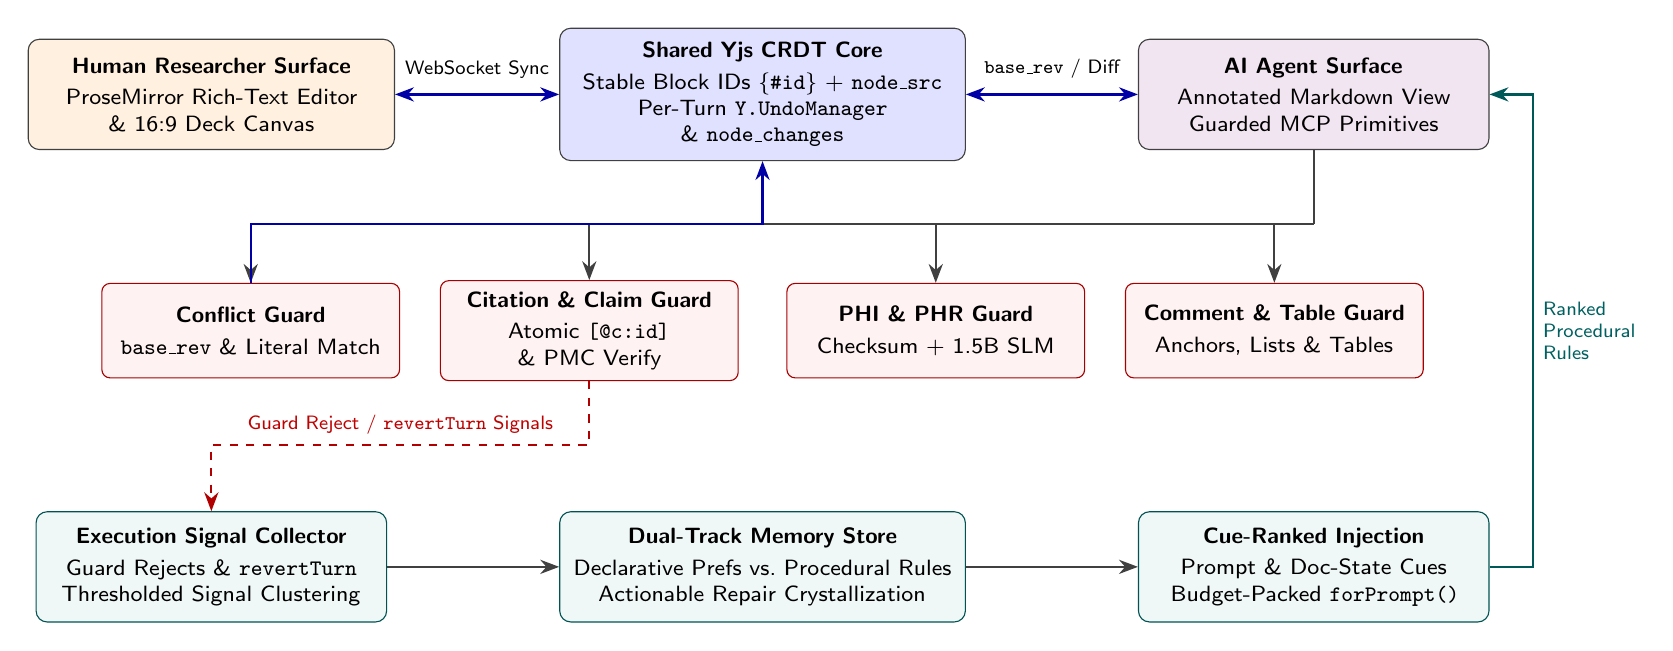
\begin{tikzpicture}[
  font=\sffamily\footnotesize,
  box/.style={draw=black!75, rounded corners=4pt, fill=white, align=center, minimum height=1.4cm, inner sep=5pt},
  guard/.style={draw=red!65!black, fill=red!5, rounded corners=3pt, align=center, text width=3.5cm, minimum height=1.2cm, inner sep=4pt},
  evol/.style={draw=teal!65!black, fill=teal!6, rounded corners=4pt, align=center, minimum height=1.4cm, inner sep=5pt},
  arr/.style={-{Stealth[length=2.4mm]}, thick, draw=black!75},
  darr/.style={{Stealth[length=2.4mm]}-{Stealth[length=2.4mm]}, thick, draw=blue!65!black}
]

% Top Layer: Dual Surface (y = 6.0)
\node[box, fill=orange!12, text width=4.3cm] (human) at (0, 6.0) {\textbf{Human Researcher Surface}\\[2pt]ProseMirror Rich-Text Editor\\\& 16:9 Deck Canvas};
\node[box, fill=blue!12, text width=4.8cm] (crdt) at (7.0, 6.0) {\textbf{Shared Yjs CRDT Core}\\[2pt]Stable Block IDs \texttt{\{\#id\}} + \texttt{node\_src}\\Per-Turn \texttt{Y.UndoManager} \& \texttt{node\_changes}};
\node[box, fill=violet!10, text width=4.1cm] (agentview) at (14.0, 6.0) {\textbf{AI Agent Surface}\\[2pt]Annotated Markdown View\\Guarded MCP Primitives};

\draw[darr] (human.east) -- node[above, font=\sffamily\scriptsize, yshift=2pt]{WebSocket Sync} (crdt.west);
\draw[darr] (crdt.east) -- node[above, font=\sffamily\scriptsize, yshift=2pt]{\texttt{base\_rev} / Diff} (agentview.west);

% Middle Layer: Pre-Write Structural Guards (y = 3.0)
\node[guard] (g1) at (0.5, 3.0) {\textbf{Conflict Guard}\\[2pt]\texttt{base\_rev} \& Literal Match};
\node[guard] (g2) at (4.8, 3.0) {\textbf{Citation \& Claim Guard}\\[2pt]Atomic \texttt{[@c:id]} \& PMC Verify};
\node[guard] (g3) at (9.2, 3.0) {\textbf{PHI \& PHR Guard}\\[2pt]Checksum + 1.5B SLM};
\node[guard] (g4) at (13.5, 3.0) {\textbf{Comment \& Table Guard}\\[2pt]Anchors, Lists \& Tables};

% Bus from AI Agent Surface down to the 4 Pre-Write Guards
\coordinate (bus_top) at (14.0, 4.35);
\draw[thick, draw=black!75] (agentview.south) -- (bus_top);
\draw[arr] (bus_top) -| (g1.north);
\draw[arr] (bus_top) -| (g2.north);
\draw[arr] (bus_top) -| (g3.north);
\draw[arr] (bus_top) -| (g4.north);

% Validated commit arrow from Conflict Guard up to Shared Yjs CRDT Core
\draw[arr, draw=blue!65!black] (g1.north) -- ++(0, 0.75) -| (crdt.south);

% Bottom Layer: Self-Evolving Procedural Memory (y = 0.0)
\node[evol, text width=4.1cm] (l1) at (0, 0.0) {\textbf{Execution Signal Collector}\\[2pt]Guard Rejects \& \texttt{revertTurn}\\Thresholded Signal Clustering};
\node[evol, text width=4.8cm] (l2) at (7.0, 0.0) {\textbf{Dual-Track Memory Store}\\[2pt]Declarative Prefs vs.\ Procedural Rules\\Actionable Repair Crystallization};
\node[evol, text width=4.1cm] (l3) at (14.0, 0.0) {\textbf{Cue-Ranked Injection}\\[2pt]Prompt \& Doc-State Cues\\Budget-Packed \texttt{forPrompt()}};

\draw[arr] (l1.east) -- (l2.west);
\draw[arr] (l2.east) -- (l3.west);

% Signal feedback from Guards to Signal Collector
\draw[arr, dashed, draw=red!70!black] (g2.south) -- (4.8, 1.55) -| node[pos=0.25, above, font=\sffamily\scriptsize, text=red!75!black]{Guard Reject / \texttt{revertTurn} Signals} (l1.north);

% Utility-ranked context feedback from Cue-Ranked Injection up to AI Agent Surface
\draw[arr, draw=teal!70!black] (l3.east) -- ++(0.55,0) |- node[pos=0.25, right, font=\sffamily\scriptsize, text=teal!75!black, align=left]{Ranked\\Procedural\\Rules} (agentview.east);

\end{tikzpicture}%
}
\caption{System architecture of Heurion 2.0, a contract-guarded clinical research and scientific authoring platform. Top: Human researchers and AI agents co-edit a shared Yjs CRDT document and slide core through synchronized surface projections (ProseMirror rich-text/deck canvas and Annotated Markdown MCP tools). Middle: All AI mutations pass through deterministic pre-write structural guards (Conflict Guard, Citation \& Claim Guard, PHI \& PHR Guard, and Comment \& Table Guard) before committing to the CRDT state. Bottom: Runtime guard rejections and human turn reverts feed a dual-track self-evolving procedural memory pipeline that crystallizes actionable repair rules and dynamically injects context-relevant directives into future turns.}
\label{fig:architecture}
\end{figure}

Heurion 2.0 is built around three core design principles:
\begin{enumerate}[leftmargin=1.5em,itemsep=2pt]
  \item \textbf{Pre-Write Structural Safety:} Every batch of AI edit operations is validated against the current CRDT document state \emph{before} any change is committed. If any operation in a batch targets a block modified by a human since the agent's read revision (\texttt{conflict\_user\_edited}), modifies a block holding an unresolved clinician track-changes suggestion (\texttt{pending\_suggestion}), fails unique literal substring matching (\texttt{text\_not\_found} or \texttt{ambiguous\_match}), drops open review-comment anchors without explicit acknowledgement (\texttt{anchor\_has\_open\_comments}), violates list or merged-table structure (\texttt{invalid\_structure} or \texttt{cell\_not\_found}), or injects unregistered raw citations (\texttt{citation\_not\_registered}), the entire batch is atomically rejected prior to mutating the document, returning the diagnostic code, repair hint, and latest block snapshot.
  \item \textbf{Local-First Clinical Privacy Boundary:} Raw clinical notes are scrubbed inside the local environment before reaching external LLM APIs: Stage~1 deterministically masks structured and checksummed identifiers in sub-millisecond time, and Stage~2 invokes a local $1.5\text{B}$ small language model on \texttt{127.0.0.1} paired with a deterministic biomedical post-validator to mask residual narrative names and addresses without over-redacting clinical terminology.
  \item \textbf{Declarative--Procedural Memory Separation:} Subjective authoring preferences (declarative memory, e.g., statistical reporting style or spelling conventions) require explicit clinician confirmation in the user interface before activation, whereas objective operational rules for navigating pre-write guards and avoiding turn reverts (procedural memory) evolve automatically from runtime execution signals without polluting declarative memory or requiring manual curation.
\end{enumerate}

% ============================================================================
% 3. DUAL-SURFACE CO-EDITING & ORIGINAL-SLICE DOCUMENT ENGINE
% ============================================================================
\section{Dual-Surface Co-Editing and Original-Slice Document Engine}
\label{sec:dualsurface}

How can autonomous AI agents edit complex Word (\texttt{.docx}) manuscripts and PowerPoint (\texttt{.pptx}) presentation decks without corrupting journal-template formatting or overwriting concurrent human edits? A central architectural observation in Heurion 2.0 is that Office Open XML (\texttt{.docx} and \texttt{.pptx}) files are delivery formats, not collaborative editing data structures. When an agent edits a \texttt{.docx} file on disk via a Python script while a human views the document in a browser, the two actors operate on divergent state representations. Heurion 2.0 eliminates this divergence by replacing direct file scripting with a Contract-Guarded Dual-Surface CRDT Engine \cite{shapiro2011crdt,kleppmann2019localfirst}.

\subsection{Shared CRDT Core with Lifecycle-Stable Block Addressing}
In Heurion 2.0, every manuscript and presentation deck resides in a server-authoritative Yjs CRDT document (\texttt{Y.Doc}) backed by SQLite state snapshots and an append-only revision log (\texttt{doc\_commits}). Every block-level ProseMirror node (heading, paragraph, list item, table, figure, or slide element) is assigned a short, lifecycle-stable identifier (\texttt{attrs.id}, rendered as \texttt{\{\#id\}}). When a human splits a paragraph or pastes content in the browser, the server-side \texttt{flush()} handler automatically detects duplicate or missing block IDs and assigns fresh unique IDs inside a system CRDT transaction, ensuring the addressing space remains bijective.

From this single CRDT core, Heurion 2.0 projects two synchronized surfaces:
\begin{enumerate}[leftmargin=1.5em,itemsep=2pt]
  \item \textbf{Human Surface:} A real-time collaborative ProseMirror rich-text editor (for manuscripts) and an interactive 16:9 SVG/HTML slide canvas (for decks) synchronized via WebSocket (\texttt{y-protocols/sync}).
  \item \textbf{Agent Surface:} A compact \emph{Annotated Markdown} view generated on demand via \texttt{doc\_read} and \texttt{slide\_read}. Each block is suffixed with its stable address \texttt{\{\#id\}}, inline citations are rendered as atomic tokens \texttt{[@c:cite\_id]}, figures as \texttt{![alt](asset:id)}, and active inline review comments as \texttt{\{\#c:comment\_id\}}.
\end{enumerate}

\subsection{Node-Level Conflict Guards and Minimal-Diff Fragment Updates}
To prevent an AI turn in Heurion 2.0 from overwriting concurrent human edits, every \texttt{doc\_edit} call specifies the \texttt{base\_rev} read by the agent. The platform queries the \texttt{node\_changes} index for all blocks modified by human actors since \texttt{base\_rev}:
\begin{itemize}[leftmargin=1.5em,itemsep=2pt]
  \item \textbf{Block-Level Structural Operations (\texttt{replace\_block}, \texttt{delete}):} If a target block has been modified by a human since \texttt{base\_rev}, the operation is rejected with error code \texttt{conflict\_user\_edited}, returning the human's latest block markdown so the agent can adapt. Similarly, blocks carrying unresolved track-changes suggestions are protected by the \texttt{pending\_suggestion} guard, and blocks holding open review comments require either preserving the comment anchors or explicitly declaring \texttt{drop\_anchors} (\texttt{anchor\_has\_open\_comments}).
  \item \textbf{Substring Replacement (\texttt{replace\_text}):} For surgical phrase edits within a paragraph, the literal \texttt{find} substring acts as its own optimistic concurrency guard: if the human edited a different sentence in the same paragraph, \texttt{find} still matches uniquely and succeeds; if the human altered the target phrase itself or if \texttt{find} matches multiple occurrences, validation fails cleanly with \texttt{text\_not\_found} or \texttt{ambiguous\_match}.
  \item \textbf{Mark-Preserving Minimal Diffs:} Notably, \texttt{replace\_text} does not re-parse the paragraph from plain text (which would destroy inline bold/italic spans, \texttt{[@c:id]} citation nodes, and comment highlights outside the matched range). Instead, it locates the matched character span in the ProseMirror node's flattened text stream and replaces only that slice, after which \texttt{writeFragment} updates only the modified XML children between the common prefix and suffix in the underlying \texttt{Y.XmlFragment}.
\end{itemize}

\subsection{Per-Turn Selective Undo in CRDT Space (\texttt{revertTurn})}
In collaborative scientific writing, a researcher may ask the AI to revise three sections, continue manually editing Section~2, and subsequently decide to undo the AI's changes. Global linear undo (\texttt{Ctrl+Z} or version rollback) would destroy the researcher's manual edits in Section~2.

Heurion 2.0 solves this via a two-tier \emph{Per-Turn Selective Undo} mechanism (\texttt{revertTurn}):
\begin{enumerate}[leftmargin=1.5em,itemsep=2pt]
  \item \textbf{In-Memory CRDT Origin Tracking:} When an AI turn commits changes to a document, the runtime tags every CRDT transaction with the turn's unique origin identifier and attaches a turn-scoped \texttt{Y.UndoManager} tracking only that origin. Invoking \texttt{revertTurn(docId, turnId)} executes \texttt{undo()} solely on the CRDT items inserted or deleted during that AI turn, leaving concurrent human character insertions---even within the same paragraph---intact.
  \item \textbf{Persistent Node-Level Fallback across Server Restarts:} Before a turn's first write, the runtime persists the pre-turn Yjs state vector in \texttt{turn\_doc\_bases}. If the server restarts before \texttt{revertTurn} is invoked, the engine reconstructs the pre-turn document tree, computes the per-block diff against the turn's recorded \texttt{node\_changes}, reverts all AI-modified blocks untouched by the user since the turn began, and safely skips blocks subsequently edited by the user (returning their IDs in \texttt{skipped}).
\end{enumerate}

\subsection{Original-Slice OOXML Patch Export}
Clinical manuscripts are frequently imported from journal-specific Word templates containing custom styles, headers/footers, macros, and embedded vector objects. During \texttt{.docx} or \texttt{.pptx} import, Heurion 2.0 stores the original archive in \texttt{doc\_packages} and records the raw XML slice (\texttt{<w:p>} or \texttt{<w:tbl>}) of every imported block in \texttt{node\_src} keyed by block ID. Upon export (\texttt{docx-export.ts}, \texttt{pptx-export.ts}), any block whose ProseMirror node is structurally equal (\texttt{node.eq(baselineNode)}, meaning its text, inline formatting marks, and attached comment range markers are unchanged) to its imported baseline is written back using its exact original \texttt{node\_src} XML bytes; only blocks whose text or inline comment/mark structure was mutated during the session are re-serialized, preserving paragraph properties (\texttt{<w:pPr>}), run fonts, and paragraph identifiers (\texttt{w14:paraId}) from the original template.

% ============================================================================
% 4. CITATION-GROUNDED EVIDENCE LOOP & CLINICAL SANDBOX
% ============================================================================
\section{Citation-Grounded Evidence Loop and Privacy-Preserving Clinical Pipeline}
\label{sec:evidence}

How can a clinical authoring platform prevent LLM citation fabrication while protecting patient privacy (PHI) in medical records? Heurion 2.0 addresses both requirements through deterministic pre-write syntactic guards and a two-stage neuro-symbolic PHI redaction funnel.

\subsection{Syntactic Citation Guard and Atomic Citation Nodes}
To prevent fabricated references from entering manuscript text, Heurion 2.0 blocks agents from writing raw bibliographic identifiers or hand-numbered brackets in prose. During pre-write validation in \texttt{OpService}, every candidate text string is scanned against structural regular expressions detecting bare DOIs (\texttt{10.\textbackslash d\{4,9\}/\dots}), bare PMIDs (\texttt{PMID:\textbackslash s*\textbackslash d+}), or unlinked reference markers. Any violation triggers \texttt{citation\_not\_registered} before modifying the document.

Instead, the agent must invoke \texttt{insert\_citation}, which queries live metadata APIs (Crossref, NCBI PubMed E-utilities, and OpenAlex), verifies the record's existence, stores the canonical metadata (authors, title, journal, year, volume, pages, DOI/PMID) in the document's \texttt{citations} table, and returns a registered token \texttt{[@c:cite\_id]}. In ProseMirror, \texttt{[@c:cite\_id]} is parsed into an atomic inline node (\texttt{atom: true}) that dynamically numbers itself according to citation order and automatically compiles the terminal References section.

\subsection{System Context: Claim Verification and Biostatistical Sandbox}
In addition to the pre-write citation guard evaluated in Section~\ref{sec:evaluation}, the platform includes a multi-agent claim verification service (\texttt{ClaimService.verify}) and a sandboxed biostatistical execution toolchain (included here for architectural context; clinician-graded evaluation of these modules is left to future work). Briefly, \texttt{verify\_claims} segments manuscript blocks into sentences, retrieves PubMed abstracts and available PubMed Central (PMC) full texts for cited \texttt{[@c:cite\_id]} records, and classifies quantitative assertions into four verdicts (\texttt{supported}, \texttt{contradicted}, \texttt{unsupported}, or \texttt{uncited\_stat}), attaching problematic claims as inline ProseMirror review comments. For statistical analysis, computation is delegated to isolated Python/R tools (\texttt{biostatistician} subagent) rather than free-text LLM arithmetic.

\subsection{Multi-Tenant PHI Redaction Funnel}
To bridge clinical data management and manuscript authoring without exposing patient identities \cite{stubbs2015deid,norgeot2020philter,presidio2021}, Heurion 2.0 enforces four privacy safeguards:
\begin{itemize}[leftmargin=1.5em,itemsep=2pt]
  \item \textbf{Per-Tenant Database Isolation \& Envelope Encryption:} Each organization tenant operates on a physically isolated SQLite database file (\texttt{tenants/<org\_id>/platform.db}) with per-tenant Data Encryption Keys (DEKs) wrapped by a master Key Encryption Key (KEK).
  \item \textbf{Two-Stage Neuro-Symbolic PHI Funnel (\texttt{phi-scan.ts}):} Using an external cloud LLM to inspect raw clinical text for PHI creates a privacy paradox: sending unredacted patient records to a third-party API in order to redact them already violates tenant data-residency boundaries. Conversely, running a frontier-scale $70\text{B}+$ parameter model on-premise imposes high GPU requirements for clinical research teams. Heurion 2.0 addresses this trade-off through a task-decomposed, two-stage neuro-symbolic funnel that operates within the local environment:
  \begin{enumerate}[leftmargin=1.5em,itemsep=1pt]
    \item \emph{Stage~1 --- Sub-Millisecond Deterministic Checksum \& Subtype Rules (\texttt{scanPhi}/\allowbreak\texttt{redactPhi}):} Deterministic rules execute first ($0.011\,\text{ms}$ per note) to validate and mask mathematically structured or field-labeled identifiers: 18-digit national IDs (ISO~7064 MOD~11-2 checksum + calendar bounds), settlement/bank cards (ISO/IEC~7812 industry prefix + Luhn mod-10 checksum with DOI/URL boundary exclusion), 11-digit mobile numbers, medical record numbers, and co-occurring patient-name + clinical diagnosis pairs spanning both pure-CJK and mixed alphanumeric/Roman-numeral subtypes (e.g., Type-2 diabetic nephropathy, diffuse large B-cell lymphoma).
    \item \emph{Stage~2 --- Pre-Masked Local Small Language Model with Symbolic Output Guard (\texttt{create\allowbreak LocalSlm\allowbreak PhiDetector} + \texttt{redact\allowbreak Phi\allowbreak Cascaded}):} Because Stage~1 pre-masks structured identifiers before Stage~2 is invoked, the Stage-2 model does not receive raw national IDs, phone numbers, or bank cards, and does not need to perform arithmetic checksum verification. Instead, a compact $1.5\text{B}$-parameter local small language model (\texttt{qwen2.5:1.5b}, $986\,\text{MB}$, served via local Ollama and gated by \texttt{assert\allowbreak Local\allowbreak PhiEndpoint} to allow only loopback \texttt{127.0.0.1}/\texttt{::1} or RFC~1918 private intranet hosts) extracts open-vocabulary residual spans in free-form ward-round narratives: unlabeled person/relative names (\texttt{unlabeled\_\allowbreak person\_\allowbreak name}) and specific residential/workplace addresses (\texttt{address\_\allowbreak or\_\allowbreak org}). Finally, a deterministic post-validator (\texttt{normalize\allowbreak AndValidate\allowbreak Stage2Entity}) verifies exact substring presence in the source text, strips kinship/location prepositions, checks Chinese family-surname membership and medical-suffix exclusions for names, and requires spatial/organizational markers for addresses---filtering out small-model hallucinations and clinical-term false positives. The model thus acts as a candidate generator and the post-validator decides what is masked; text containing no CJK characters (e.g., English manuscript prose) is not sent to the model.
  \end{enumerate}
  \item \textbf{Pseudonymous Subject Mapping \& PHR Red-Lines:} Within research cohorts, real patient identifiers are replaced by pseudonymous subject codes (\texttt{P001}, \texttt{P002}, \dots) via an in-memory translation table. Furthermore, a dedicated Personal Health Record guard (\texttt{phr\_guard}) enforces read-only access on patient-uploaded primary medical records, preventing AI tools from altering ground-truth clinical evidence.
  \item \textbf{Regulatory Scope:} These mechanisms reduce exposure but do not by themselves establish compliance with either PIPL or HIPAA. Pseudonymous subject codes are de-identification rather than anonymization: under PIPL, data that can be re-linked with a retained mapping table remains personal information \cite{pipl2021}. The current scanner implements mainland Chinese identifier formats (resident ID numbers, mobile numbers, hospital record numbers, Chinese surnames/addresses); it does not yet cover HIPAA Safe Harbor identifiers such as Social Security numbers, U.S.-format telephone numbers, full dates, or English geographic subdivisions \cite{hipaa1996}, so U.S. deployment requires extending it.
\end{itemize}

% ============================================================================
% 5. DUAL-TRACK SELF-EVOLVING PROCEDURAL MEMORY
% ============================================================================
\section{Dual-Track Self-Evolving Procedural Memory}
\label{sec:evolution}

A recurring challenge in contract-guarded agent environments is helping the LLM internalize operational boundaries without manual prompt engineering. When an agent's tool call is blocked by a pre-write guard or reverted by a user, how does the system help the agent adapt both within the current turn and across future authoring sessions?

As shown in the bottom tier of Figure~\ref{fig:architecture}, Heurion 2.0 combines intra-turn pre-flight validation probes with a cross-session dual-track procedural memory pipeline:

\subsection{Intra-Turn Pre-Flight Probe (\texttt{doc\_validate} \& \texttt{dry\_run})}
Within a single turn, agents in Heurion 2.0 can invoke \texttt{doc\_validate} (or pass \texttt{dry\_run: true} to \texttt{doc\_edit}) prior to committing complex multi-block edits. The probe executes the full suite of conflict guards, citation registration checks, anchor integrity checks, and post-edit structural diffs against an ephemeral in-memory clone of the ProseMirror document tree without incrementing \texttt{rev}, mutating the Yjs CRDT state, or polluting the undo stack. If a violation is detected, the probe returns \texttt{\{valid: false, code, hint, current\}}, enabling immediate self-correction within the same reasoning turn.

\subsection{Dual-Track Memory Separation and Actionable Rule Crystallization}
Across sessions, Heurion 2.0 prevents memory pollution by physically separating declarative preferences from procedural rules:
\begin{itemize}[leftmargin=1.5em,itemsep=2pt]
  \item \textbf{Track A --- Declarative Memory (\texttt{MemoryService}):} Captures domain conventions and author preferences (e.g., ``Always report continuous skewed variables as median (IQR)'', ``Use British English spelling''). Because stylistic preferences are subjective, newly extracted items enter a \texttt{candidate} state and require explicit human approval in the UI before becoming \texttt{confirmed}.
  \item \textbf{Track B --- Procedural Harness Memory (\texttt{ProceduralHarnessService}):} Captures objective operational rules for navigating guards, tools, and specialist subagents within each user's isolated namespace (\texttt{ownerId}). Whenever \texttt{OpService} rejects an AI edit or a user invokes \texttt{revertTurn}, the \texttt{ExecutionSignals} collector automatically logs a structured runtime signal (recording the document ID, turn ID, signal kind, guard code, and diagnostic detail) into the \texttt{execution\_signals} table.
\end{itemize}

At the end of an authoring session, \texttt{evolveFromSignals()} groups unconsumed execution signals by signal kind and guard code. Any failure pattern occurring at least twice either increments the evidence counter of an existing procedural rule or crystallizes a new active procedural directive via guard-specific actionable templates (\texttt{LEARNED\_RULE\_TEMPLATES})---requiring zero manual UI intervention. Rather than emitting generic warnings (e.g., ``call \texttt{doc\_validate} before editing''), each crystallized rule encodes the exact positive parameter or tool-sequencing fix required by the underlying contract (e.g., including leading clause context or explicit \texttt{occurrence: 2} for \texttt{ambiguous\_match}; stripping HTML \texttt{<sup>}/\texttt{<sub>} tags from \texttt{find} while retaining them in \texttt{replace} for \texttt{text\_not\_found}; prepending \texttt{\{op:\ "move"\}} before \texttt{\{op:\ "merge"\}} in the same batch for \texttt{invalid\_structure}; calling \texttt{comments\_list} after \texttt{doc\_read} and passing \texttt{ack\_comments} + \texttt{comment\_reply} for \texttt{anchor\_has\_open\_comments}; targeting only the top-left origin \texttt{\{row:\ 0, col:\ 0\}} of merged table headers for \texttt{cell\_not\_found}; and restricting edits to the single named block after \texttt{user\_reverted\_turn}).

\subsection{Context-Aware Cue Ranking and Prompt Budget Packing}
Injecting all procedural rules into every turn would waste context tokens. Before each turn, \texttt{ProceduralHarnessService\allowbreak.forPrompt()} scores each active rule in the user's store by combining its historical evidence count with two context cues (since guard codes themselves never appear in a user's natural-language request): (1) a \emph{message cue} matching task keywords in the user's prompt (e.g., DOI/PMID or citation terms for \texttt{citation\_not\_registered}, replacement/statistic verbs for \texttt{ambiguous\_match} and \texttt{text\_not\_found}, paragraph-merge or transition verbs for \texttt{invalid\_structure} and \texttt{user\_reverted\_turn}), and (2) a \emph{document-state cue} inspected from the current document (human edits within the last two revisions for \texttt{conflict\_user\_edited}, open comment threads for \texttt{anchor\_has\_open\_comments}, pending suggestions for \texttt{pending\_suggestion}, or the presence of a table for \texttt{cell\_not\_found} and \texttt{invalid\_table}). Specifically, each rule receives $0.1$ points per historical occurrence, $+5$ points when its message cue matches the user prompt, and $+8$ points when its document-state cue is active in the target manuscript (heuristic weights set prior to evaluation). Rules are sorted by score and greedily packed up to at most $4$ rules within a $1,000$-character budget. To isolate rule content from prompt-length effects in controlled experiments, the service also supports a \texttt{placebo} mode (\texttt{PROCEDURAL\_MODE=placebo}) that appends a length-matched block of generic platform background text alongside the static baseline rules. In multi-tenant deployments, an optional background service (\texttt{HarnessEvolutionService}) can also periodically distill high-frequency rules across tenants into a shared profile overlay (\texttt{evolved.cordis.yml}).

% ============================================================================
% 6. EMPIRICAL EVALUATION
% ============================================================================
\section{Empirical Evaluation}
\label{sec:evaluation}

We evaluate Heurion 2.0 through a two-tier, two-generation empirical protocol (\texttt{ANALYSIS\_\allowbreak PLAN.md} for v1 and \texttt{ANALYSIS\_\allowbreak PLAN\_\allowbreak v2.md} for v2) combining:
\begin{enumerate}[leftmargin=1.5em,itemsep=2pt]
  \item \textbf{Deterministic and Local-SLM Benchmarks (\texttt{run\_eval.ts} \& \texttt{v2/phi/run.ts}):} $1,010$ evaluation records against the platform's TypeScript/\allowbreak SQLite/\allowbreak Yjs engine and local Ollama runtime, comprising $50$ CRDT concurrency/revert trials (\texttt{exp1}), $660$ initial citation and template PHI guard records (\texttt{exp2b}), and a locked $300$-record multi-specialty Chinese clinical PHI de-identification test split (\texttt{v2-phi}: $100$ diverse clinical notes containing $745$ PHI spans [$485$ narrative, $260$ labeled] and $200$ hard-negative clinical sentences evaluated across $4$ ablation arms). Local Stage-2 PHI extraction used \texttt{qwen2.5:\allowbreak 1.5b} ($986\,\text{MB}$, Ollama v0.20.5 on \texttt{http://\allowbreak 127.0.0.1:\allowbreak 11434/\allowbreak api/\allowbreak chat}, \texttt{temperature=0}, \texttt{format='json'}).
  \item \textbf{Pre-Specified Live LLM Evaluations (\texttt{ANALYSIS\_PLAN.md} \& \texttt{ANALYSIS\_PLAN\_v2.md}):} $10,769$ analysed live agent turns across $20$ open-access (CC~BY) clinical research manuscripts from PubMed Central (PMC), comprising: (i) $1,241$ v1 baseline turns ($162$ in \texttt{exp2a-papers} and $1,079$ in \texttt{exp3}); (ii) $4,488$ three-arm collaborative manuscript editing turns in \texttt{v2-q1} ($2,148$ development turns in Phase~1a on $10$ PMC manuscripts and $2,340$ confirmatory turns in Phase~1b on $10$ newly selected 2026 PMC manuscripts across stress, multi-turn session, and routine tasks); and (iii) $5,040$ longitudinal procedural memory turns in \texttt{v2-exp3} ($432$ pilot turns across $3$ arms and $4,608$ confirmatory turns across $4$ arms $\times$ $16$ users $\times$ $8$ sessions $\times$ $9$ uncovered constraint tasks, with $0$ failed or excluded turns). All online turns were executed using model ID \texttt{deepseek-flash} via \texttt{@deepseek-ai/\allowbreak dsh-sdk-client} against \texttt{https://api.deepseek.com/\allowbreak anthropic/v1}. Across longitudinal memory experiments, each turn executes in a fresh agent session and each simulated user evolves within an isolated per-user procedural memory namespace (\texttt{ownerId}) without cross-user rule sharing, ensuring that all user trajectories remain statistically independent.
\end{enumerate}

\subsection{Experiment 1: Dual-Surface CRDT Engine vs.\ Script-Based File Mutation}
Table~\ref{tab:v1_vs_v2} contrasts the architectural mechanisms of direct script mutation (\texttt{python-docx}), script mutation paired with post-hoc file auditing, and Heurion 2.0.

\paragraph{Experiment 1a: Deterministic Engine Micro-Benchmarks (\texttt{exp1}).}
Table~\ref{tab:v2_bench} reports in-process micro-benchmarks of Heurion 2.0 over $N=50$ trials on a six-block \texttt{.docx} clinical protocol template (one styled heading, a bold paragraph, an italic paragraph, two list items, and a plain paragraph). In each trial, an AI turn applies two \texttt{replace\_text} edits ($p_1, p_2$), a simulated human edits a different phrase inside $p_2$, a stale \texttt{replace\_block} is probed, and the AI turn is selectively reverted via \texttt{revertTurn}. All $50/50$ trials reproduced the original \texttt{<w:p>} XML bytes of the untouched heading and final paragraph verbatim via \texttt{node\_src}, rejected the stale overwrite with \texttt{conflict\_user\_edited}, and undid the AI edits while preserving the human's intra-paragraph edit in $p_2$ at sub-millisecond latency ($0.168\,\text{ms}$ validation, $0.338\,\text{ms}$ edit, $0.129\,\text{ms}$ revert).

\begin{table}[t]
\centering
\caption{Architectural mechanism comparison across direct script mutation (\texttt{python-docx}), script mutation with post-hoc file auditing, and Heurion 2.0's contract-guarded dual-surface CRDT architecture. Entries describe system design mechanisms, not measured rates.}
\label{tab:v1_vs_v2}
\vspace{2pt}
\resizebox{\textwidth}{!}{%
\begin{tabular}{@{}lccc@{}}
\toprule
\textbf{Dimension} & \textbf{Direct Script (\texttt{python-docx})} & \textbf{Script + Post-Hoc Audit} & \textbf{Heurion 2.0 (Ours)} \\
\midrule
Source of Truth & Raw \texttt{.docx} on Disk & Raw \texttt{.docx} + Derived Projection & \textbf{Shared Yjs CRDT + SQLite} \\
Block Addressing & None (Regex/XPath) & File-Native \texttt{w14:paraId} / Shape ID & \textbf{Server-Assigned \texttt{\{\#id\}}} \\
Export of Untouched Blocks & Full Re-serialization & Whole-File Save & \textbf{Original XML Slice (\texttt{node\_src})} \\
Concurrent Human Edits & Silent Overwrite & Post-Hoc Node-Level 3-Way Merge & \textbf{Pre-Write \texttt{base\_rev} Guard} \\
Undo of One AI Turn & Unsupported & File-Level Rollback & \textbf{Per-Turn \texttt{Y.UndoManager}} \\
Unregistered Citations & Not Checked & Post-Write Audit & \textbf{Pre-Write Block} \\
Pre-Flight Validation & None & Subprocess Audit Script & \textbf{In-Memory Dry Run} \\
\bottomrule
\end{tabular}%
}
\end{table}

\begin{table}[t]
\centering
\caption{Heurion 2.0 dual-surface CRDT engine micro-benchmark results (\texttt{exp1}) over $N=50$ trials on the synthetic clinical protocol template. Latencies are wall-clock means of in-process calls on a single developer machine.}
\label{tab:v2_bench}
\vspace{2pt}
\begin{tabular}{@{}lc@{}}
\toprule
\textbf{Metric} & \textbf{Result} \\
\midrule
Untouched blocks reproduced verbatim on export (heading + final paragraph) & $50/50$ \\
Stale \texttt{replace\_block} rejected with \texttt{conflict\_user\_edited} & $50/50$ \\
Turn revert undoes AI edits while keeping the human edit in the same paragraph & $50/50$ \\
Mean pre-flight validation latency (\texttt{OpService.validate}) & $0.168\,\text{ms}$ \\
Mean guarded edit latency (\texttt{OpService.edit}, two ops) & $0.338\,\text{ms}$ \\
Mean per-turn revert latency (\texttt{revertTurn}) & $0.129\,\text{ms}$ \\
\bottomrule
\end{tabular}
\end{table}

\paragraph{Experiment 1b: End-to-End Clinical Manuscript Editing---Heurion 2.0 MCP vs.\ \texttt{python-docx} (\texttt{exp2a-papers}).}
To test how the two editing surfaces behave under live LLM tool use on full-length journal manuscripts, we compared Heurion 2.0's MCP surface (\texttt{PROCEDURAL\_MODE=off}) against a baseline coding agent using the same model (\texttt{deepseek-flash}) and identical authoring guidelines (\texttt{baseline.cordis.yml}) to edit \texttt{manuscript.docx} directly in a workspace directory. In the baseline arm, the agent runs inside the same \texttt{DeepSeekHarness} runtime with unrestricted \texttt{bash} and \texttt{python3} access (including \texttt{python-docx}, \texttt{zipfile}, and \texttt{xml.etree.ElementTree}) and is explicitly instructed to \emph{``preserve the existing formatting, comments and tracked changes''}. Both arms executed $3$ paired simulated user seeds ($\text{seeds } 201\text{--}203$) $\times$ $3$ PMC clinical manuscripts $\times$ $9$ authoring task archetypes (\texttt{concurrent\_edit}, \texttt{citation}, \texttt{pending\_suggestion}, \texttt{open\_comment\_anchor}, \texttt{term\_unify}, \texttt{table\_row}, \texttt{out\_of\_scope\_revert}, \texttt{p\_value\_format}, and \texttt{move\_subsection}), yielding $81$ turns per arm ($162$ turns total; $32,995$ untouched paragraphs per arm). Both arms exported standard \texttt{.docx} archives evaluated by the same OOXML inspector (\texttt{manuscripts/compare.ts}).

\begin{table}[t]
\centering
\caption{End-to-end clinical manuscript editing comparison (\texttt{exp2a-papers}, $162$ live LLM turns across $81$ paired tasks per arm, $3$ simulated user seeds $\times$ $3$ manuscripts $\times$ $9$ archetypes) between Heurion 2.0 MCP primitives and direct \texttt{python-docx} file scripting. 95\% confidence intervals use the Wilson score method; $p$-values are two-sided Fisher's exact tests. \textsuperscript{\dag}In $2$ \texttt{open\_comment\_anchor} turns (\texttt{u3-s3}, \texttt{u1-s3}), the MCP agent invoked \texttt{delegate\_task} (\texttt{fact\_checker}) without being asked to, which attached $7$ unrequested verification comments (\texttt{<w:commentRangeStart/>}) to non-target paragraphs; their text was unchanged (\texttt{content\_changed = 0}), but these are AI-initiated writes outside the task scope. \textsuperscript{\ddag}In full-paragraph rewrites, the MCP agent passed \texttt{drop\_anchors: true} ($6/9$ cases) to clear obsolete range tags after replying to all $9/9$ review threads via \texttt{comment\_reply}, whereas \texttt{python-docx} run-level edits left the sibling \texttt{<w:commentRangeStart/>} tags in place without replying to \texttt{word/comments.xml}.}
\label{tab:exp2a_papers}
\vspace{2pt}
\resizebox{\textwidth}{!}{%
\begin{tabular}{@{}lccc@{}}
\toprule
\textbf{Evaluation Endpoint} & \textbf{Heurion 2.0 MCP ($n=81$)} & \textbf{Direct \texttt{python-docx} ($n=81$)} & \textbf{Fisher $p$} \\
\midrule
Task completion rate across all 9 archetypes & $76/81$ ($93.8\%$, CI $86.4\text{--}97.3\%$) & $77/81$ ($95.1\%$, CI $88.0\text{--}98.1\%$) & $1.0000$ \\
Untouched paragraphs with unintended content changes & $0/32,995$ ($0.00\%$) & $4/32,995$ ($0.01\%$) & $0.1250$ \\
Untouched paragraphs preserved byte-identically\textsuperscript{\dag} & $32,988/32,995$ ($99.98\%$) & $32,991/32,995$ ($99.99\%$) & $0.5488$ \\
Edited paragraphs preserving native \texttt{w14:paraId} & $41/45$ ($91.1\%$, CI $79.3\text{--}96.5\%$) & $37/45$ ($82.2\%$, CI $68.7\text{--}90.7\%$) & $0.3529$ \\
Edited paragraphs preserving layout, fonts, and emphasis & $44/45$ ($97.8\%$) & $45/45$ ($100.0\%$) & $1.0000$ \\
Review comments read \& replied in thread (\texttt{acknowledged}) & $\mathbf{9/9}$ ($\mathbf{100.0\%}$, CI $70.1\text{--}100\%$) & $0/9$ ($0.0\%$, CI $0.0\text{--}29.9\%$) & $\mathbf{<0.0001}$ \\
Inline \texttt{<w:commentRangeStart/>} tag retained ($6/9$ cleared via \texttt{drop\_anchors})\textsuperscript{\ddag} & $3/9$ ($33.3\%$, CI $12.1\text{--}64.6\%$) & $\mathbf{9/9}$ ($\mathbf{100.0\%}$, CI $70.1\text{--}100\%$) & $\mathbf{0.0090}$ \\
Clinician pending track-change suggestion preserved & $9/9$ ($100.0\%$, CI $70.1\text{--}100\%$) & $9/9$ ($100.0\%$, CI $70.1\text{--}100\%$) & $1.0000$ \\
Unregistered bare DOI / PMID injected into manuscript body & $0/81$ ($0.0\%$, CI $0.0\text{--}4.5\%$) & $1/81$ ($1.2\%$, CI $0.2\text{--}6.7\%$) & $1.0000$ \\
\bottomrule
\end{tabular}%
}
\end{table}

Table~\ref{tab:exp2a_papers} summarizes three empirical observations from \texttt{exp2a-papers}:
\begin{enumerate}[leftmargin=1.5em,itemsep=2pt]
  \item \textbf{Comparable Task Completion and Structural Preservation Rates:} Task completion did not differ significantly between Heurion 2.0 MCP ($76/81 = 93.8\%$) and direct \texttt{python-docx} scripting ($77/81 = 95.1\%$, Fisher $p = 1.0000$). Across $32,995$ non-target paragraphs, Heurion 2.0 produced $0$ unintended text modifications compared to $4$ altered non-target paragraphs in the \texttt{python-docx} arm ($p = 0.1250$), and retained \texttt{w14:paraId} on $41/45$ ($91.1\%$) vs.\ $37/45$ ($82.2\%$, $p = 0.3529$) edited paragraphs; neither difference reached statistical significance at $n=81$ turns per arm. Why were $7$ of $32,995$ untouched paragraphs in Heurion 2.0 not byte-identical ($32,988/32,995 = 99.98\%$ vs.\ $32,991/32,995 = 99.99\%$)? Inspection of the turn logs showed that all $7$ paragraphs occurred in two \texttt{open\_comment\_anchor} turns (\texttt{u3-s3} on \texttt{PMC8861838}, $4$ paragraphs; \texttt{u1-s3} on \texttt{PMC10260499}, $3$ paragraphs) where the MCP agent voluntarily invoked the \texttt{fact\_checker} subagent (\texttt{delegate\_task}), which attached unrequested \texttt{<w:commentRangeStart/>} verification comments to those $7$ paragraphs while leaving their text unchanged (\texttt{content\_changed = 0}). We therefore report these as out-of-scope side effects: Heurion 2.0 made $0$ unintended text changes but $7$ unrequested comment insertions on non-target paragraphs.
  \item \textbf{Comment-Thread Resolution vs.\ Unassisted File Scripting:} In the \texttt{open\_\allowbreak comment\_\allowbreak anchor} task (which instructs the agent to rewrite a Methods paragraph according to two attached clinician review comments), although the baseline agent had full Python/XML access to \texttt{word/comments.xml}, standard \texttt{python-docx} scripts written by the agent iterated over \texttt{Document.paragraphs} (which does not expose \texttt{word/comments.xml}) and lacked a dedicated comment-thread tool or pre-write guard; consequently, the file agent modified the paragraph's text runs while leaving the sibling \texttt{<w:commentRangeStart/>} XML tags in place ($9/9$ vs.\ $3/9$, $p=0.0090$) and never appended a reply to \texttt{word/comments.xml} ($0/9$ acknowledged). Conversely, Heurion 2.0's \texttt{anchor\_has\_\allowbreak open\_comments} guard and \texttt{comments\_list}/\texttt{comment\_reply} tools prompted the MCP agent to inspect the comments, declare \texttt{drop\_anchors} when replacing the full paragraph ($6/9$ cases), and post structured replies in all $9/9$ ($100\%$, $p < 0.0001$) review threads. These replies live in the platform's comment threads: the exported \texttt{.docx} does not carry them, and in $4/9$ exported files the two original clinician comments were removed along with their anchors, so a reviewer working only in Word would not see how the comments were resolved.
  \item \textbf{Methodological Note on File-Arm Concurrent Edits:} Both arms preserved $9/9$ clinician insertions in \texttt{concurrent\_edit}. Inspection of the event logs revealed that because the file agent executes a single atomic \texttt{bash} call (\texttt{Document('manuscript.docx') ... save()}) whereas the harness callback \texttt{humanEditsFile} fires upon \texttt{tool\_result} completion, the simulated clinician insertion in the file arm occurred between separate \texttt{bash} invocations rather than mid-flight between an in-memory read and write. Mid-flight stale-snapshot overwrites are evaluated deterministically in Table~\ref{tab:v2_bench} ($50/50$ intercepted) and in Experiment~1c below.
\end{enumerate}

\paragraph{Experiment 1c: Confirmatory Three-Arm Collaborative Manuscript Editing (\texttt{v2-q1}, $4,488$ Turns).}
Because the initial $162$-turn \texttt{exp2a-papers} comparison used explicit preservation prompts, single-turn tasks, and a file baseline without literature search tools, we designed a two-phase development--validation benchmark (\texttt{ANALYSIS\_PLAN\_v2.md} \S 2--\S 4b) comparing three arms under natural clinician instructions, true mid-turn/inter-turn concurrent human edits, complex journal OOXML templates ($188/188$ fidelity checks passing in \texttt{v2/fidelity/run.ts}), and identical literature search access:
\begin{itemize}[leftmargin=1.5em,itemsep=1pt]
  \item \textbf{Arm P (Heurion 2.0 Platform):} Dual-surface CRDT core with document-scoped MCP tools ($63$ tools exposed per manuscript via \texttt{mcp/scope.ts}) and pre-write structural/citation guards.
  \item \textbf{Arm B1 (Direct File Scripting):} Coding agent with \texttt{bash}/\texttt{python3} (\texttt{python-docx}, \texttt{lxml}) editing \texttt{manuscript.docx}.
  \item \textbf{Arm B2 (Tool-Assisted File Scripting + Audit):} Same as \texttt{B1} plus helper inspection/audit scripts and the same live Crossref/PubMed/OpenAlex literature search tools as \texttt{P}.
\end{itemize}
In the \textbf{Development Phase (1a, $2,148$ turns across $10$ PMC manuscripts)}, \texttt{P} eliminated lost concurrent clinician sentences ($0$ vs.\ $23$ in \texttt{B1} and $17$ in \texttt{B2}) and OOXML structural corruption ($0$ vs.\ $32$ in \texttt{B1} and $3$ in \texttt{B2}), achieving a rework odds ratio of $\text{OR}=3.62$ vs.\ \texttt{B1} (Holm $p=2.14\times 10^{-6}$) and $20\%$ lower per-turn cost ($\text{GMR}=0.80$, $p<10^{-21}$), while exposing five platform gaps (unprotected platform-native user suggestions, lack of scoped batch text replacement, unverified citation claim support at insertion time, manual paragraph merges dropping inline marks, and stripped citation subtitles). After implementing fixes \texttt{F1}--\texttt{F5} and freezing tag \texttt{paper-eval-v2-p1b}, we executed the \textbf{Confirmatory Phase (1b, $2,340$ turns = $780$ turns/arm across $10$ newly selected 2026 CC~BY PMC manuscripts: $123$ single-turn stress tasks, $576$ multi-turn collaborative session turns [9 papers $\times$ 8 sessions $\times$ 8 turns], and $81$ routine tasks per arm)}.

\begin{table}[t]
\centering
\caption{Confirmatory Phase 1b three-arm clinical manuscript editing results (\texttt{v2-q1}, $N=2,340$ live LLM turns across $10$ unseen 2026 PMC manuscripts; $780$ paired turns per arm). Primary accuracy models use mixed-effects logistic regression on stress + multi-turn session turns ($n=699$/arm); primary cost models use linear mixed-effects regression on log-cost across all $780$ turns/arm, with Holm step-down correction across the four pre-specified confirmatory tests.}
\label{tab:v2_q1_1b}
\vspace{2pt}
\resizebox{\textwidth}{!}{%
\begin{tabular}{@{}lccccc@{}}
\toprule
\textbf{Endpoint / Stratum} & \textbf{Heurion 2.0 (\texttt{P})} & \textbf{Direct Script (\texttt{B1})} & \textbf{Assisted Script (\texttt{B2})} & \textbf{\texttt{B1} vs.\ \texttt{P} Effect (Holm $p$)} & \textbf{\texttt{B2} vs.\ \texttt{P} Effect (Holm $p$)} \\
\midrule
Stress Tasks Rework ($n=123$/arm) & $\mathbf{2.4\%}$ ($3/123$) & $20.3\%$ ($25/123$) & $9.8\%$ ($12/123$) & --- & --- \\
Multi-Turn Session Rework ($n=576$/arm) & $\mathbf{5.4\%}$ ($31/576$) & $13.4\%$ ($77/576$) & $10.6\%$ ($61/576$) & --- & --- \\
Routine Tasks Rework ($n=81$/arm) & $\mathbf{4.9\%}$ ($4/81$) & $8.6\%$ ($7/81$) & $8.6\%$ ($7/81$) & --- & --- \\
\textbf{All Turns Rework ($n=780$/arm)} & $\mathbf{4.9\%}$ ($\mathbf{38/780}$) & $14.0\%$ ($109/780$) & $10.3\%$ ($80/780$) & $\mathbf{\text{OR}=32.47}$ ($\mathbf{1.03\times 10^{-16}}$) & $\mathbf{\text{OR}=9.66}$ ($\mathbf{1.23\times 10^{-8}}$) \\
Severe Rework ($n=780$/arm) & $\mathbf{1.2\%}$ ($9/780$) & $4.4\%$ ($34/780$) & $5.4\%$ ($42/780$) & $\text{OR}=27.98$ ($p=4.20\times 10^{-6}$) & $\text{OR}=51.95$ ($p=7.87\times 10^{-8}$) \\
\midrule
Lost Human/Collaborator Content & $\mathbf{0}$ & $18$ & $22$ & --- & --- \\
OOXML File Structural Corruption & $\mathbf{1}$ & $32$ & $3$ & --- & --- \\
Out-of-Scope Collateral Edits & $\mathbf{1}$ & $9$ & $8$ & --- & --- \\
Fabricated / Mismatched Citations & $\mathbf{0}$ & $1$ & $3$ & --- & --- \\
\midrule
Total API Cost ($780$ turns/arm) & $\mathbf{\$9.26}$ & $\$13.21$ & $\$13.05$ & $\mathbf{\text{GMR}=0.70}$ ($\mathbf{3.73\times 10^{-73}}$) & $\mathbf{\text{GMR}=0.67}$ ($\mathbf{2.99\times 10^{-95}}$) \\
Median Turn Latency (Stress / Session) & $\mathbf{33.5\,\text{s} / 15.5\,\text{s}}$ & $57.3\,\text{s} / 26.5\,\text{s}$ & $61.6\,\text{s} / 27.9\,\text{s}$ & $-41.5\%$ / $-41.5\%$ & $-45.6\%$ / $-44.4\%$ \\
\bottomrule
\end{tabular}%
}
\end{table}

As shown in Table~\ref{tab:v2_q1_1b}, all four pre-specified confirmatory hypotheses in Phase~1b passed after Holm correction: Heurion 2.0 reduced rework odds by $\text{OR}=32.47$ ($95\%$ CI $14.39\text{--}73.26$, Holm $p=1.03\times 10^{-16}$) against \texttt{B1} and $\text{OR}=9.66$ ($95\%$ CI $4.43\text{--}21.08$, Holm $p=1.23\times 10^{-8}$) against \texttt{B2}, while reducing API cost by $30\%$ ($\text{GMR}=0.70$, $95\%$ CI $0.67\text{--}0.73$, Holm $p=3.73\times 10^{-73}$) and $33\%$ ($\text{GMR}=0.67$, $95\%$ CI $0.64\text{--}0.69$, Holm $p=2.99\times 10^{-95}$) and cutting median turn latency by $41\%$--$46\%$. Pre-write guards intercepted $138$ unsafe operations across $111$ platform turns, preventing any loss of concurrent human edits ($0$ vs.\ $18$ and $22$). Post-hoc root-cause inspection of all $38$ platform rework turns (\texttt{ANALYSIS\_PLAN\_v2.md} \S 5.3.4) showed that $22/38$ were evaluator oracle false positives (affecting all arms equally, e.g., body sentences starting with ``Table~1'' flagged as missing \texttt{SEQ} caption fields), leaving only $16/780$ ($2.1\%$) true platform/model defects across $6$ root causes, all of which were subsequently patched and covered by $148$ unit tests.

\subsection{Experiment 2: Pre-Write Citation and Two-Stage Neuro-Symbolic PHI Guards (\texttt{exp2b} \& Locked \texttt{v2-phi} Test Split)}

To quantify the complementary roles of Stage-1 deterministic validators (\texttt{scanPhi}/\allowbreak\texttt{redactPhi}) and the Stage-2 local small language model (\texttt{qwen2.5:1.5b} via loopback Ollama, \texttt{redact\allowbreak Phi\allowbreak Cascaded}), we first evaluated Heurion 2.0 across $660$ template test records (\texttt{exp2b}: $100$ citation-guard sentences, $200$ synthetic positive clinical notes containing $720$ PHI spans across $7$ categories, and $360$ negative controls across $4$ strata; Table~\ref{tab:guards}), and then conducted a pre-specified, single-run evaluation on a locked, multi-specialty Chinese clinical de-identification test set (\texttt{v2-phi}, Table~\ref{tab:v2_phi_test}):
\begin{enumerate}[leftmargin=1.5em,itemsep=1pt]
  \item \textbf{Unregistered Inline Citations ($N=100$ distinct sentences):} $40$ bare DOIs across $8$ biomedical publisher prefixes, $30$ \texttt{https://doi.org/} URLs, and $30$ bare PMIDs. All $100/100$ ($100\%$) were intercepted prior to CRDT mutation with \texttt{citation\_not\_registered}.
  \item \textbf{Template Verification Benchmark (\texttt{exp2b}, $720$ Spans in $200$ Notes + $360$ Negative Controls):} As shown in Table~\ref{tab:guards}, \textbf{Stage~1 alone} ($0.011\,\text{ms}$/note) achieved $100.0\%$ ($600/600$) recall across the five structured and labeled categories, $0/200$ false positives on numeric-dense PMC biostatistical paragraphs, and $0/100$ false positives on invalid-checksum 16--18 digit serials, while \textbf{Stage~2 (\texttt{qwen2.5:1.5b} + post-validator)} captured $110/120$ ($91.7\%$) of template narrative names and addresses ($710/720 = 98.6\%$ combined recall) with $1/60$ ($1.7\%$ combined across the two $30$-sentence strata: $1/30$ template and $0/30$ independent) false positives on clean Chinese clinical sentences (vs.\ $60/60$ without post-validation).
  \item \textbf{Locked Multi-Specialty Clinical De-Identification Test Set (\texttt{v2-phi}, $100$ Notes / $745$ Spans + $200$ Hard-Negative Sentences):} Because \texttt{exp2b}'s narrative clauses shared a single phrasing template, we constructed an independent benchmark (\texttt{ANALYSIS\_PLAN\_v2.md} \S 3) generated by an external LLM across diverse clinical departments and note types (admission notes, ward-round records, discharge summaries, family consultations) where $65.1\%$ ($485/745$) of PHI spans occur in unlabeled free-form narrative prose and $34.9\%$ ($260/745$) occur in labeled fields, paired with $200$ hard-negative Chinese clinical sentences dense with eponyms, anatomical terms, drug regimens, and statistical results. After refining Stage-1 surname-prefix stripping and Stage-2 biomedical exclusion lists on the \texttt{dev} split ($40$ notes + $80$ negatives), we executed a single locked run on the held-out \texttt{test} split ($100$ notes + $200$ negatives; \texttt{TEST\_RUN.lock}, Table~\ref{tab:v2_phi_test}) across four pre-specified ablation configurations:
  \begin{itemize}[leftmargin=1.2em,itemsep=1pt]
    \item \texttt{A\_stage1} (\emph{Stage-1 regex/checksum only}): Achieved $100.0\%$ ($209/209$) span precision and $0.0\%$ ($0/200$) hard-negative FPR, but recalled only $27.4\%$ ($204/745$) of total PHI---capturing $71.9\%$ ($187/260$) of labeled spans but only $3.5\%$ ($17/485$) of narrative spans ($0/360$ narrative person names, $0/99$ narrative addresses).
    \item \texttt{B\_platform} (\emph{Stage~1 + Local $1.5\text{B}$ SLM + Deterministic Post-Validator}): Raised overall PHI recall by $+59.6$ percentage points to $\mathbf{87.0\%}$ ($\mathbf{648/745}$, Wilson $95\%$ CI $84.4\text{--}89.2\%$), boosting narrative PHI recall from $3.5\%$ to $\mathbf{83.3\%}$ ($\mathbf{404/485}$, CI $79.7\text{--}86.4\%$; narrative person names $289/360 = 80.3\%$, narrative addresses $92/99 = 92.9\%$, narrative workplaces $6/7 = 85.7\%$) and labeled recall to $\mathbf{93.8\%}$ ($\mathbf{244/260}$), while maintaining $\mathbf{97.6\%}$ ($\mathbf{482/494}$, CI $95.8\text{--}98.6\%$) span precision and a $\mathbf{6.0\%}$ ($\mathbf{12/200}$, CI $3.5\text{--}10.2\%$) hard-negative sentence FPR.
    \item \texttt{C\_slm\_unvalidated} (\emph{Stage~1 + Local $1.5\text{B}$ SLM without Post-Validator}): Recalled $87.7\%$ ($653/745$) of PHI (only $+5$ spans over \texttt{B\_platform}), but suffered catastrophic over-redaction of biomedical terminology: span precision collapsed to $56.2\%$ ($487/866$) and hard-negative sentence FPR surged to $\mathbf{92.0\%}$ ($\mathbf{184/200}$).
    \item \texttt{D\_rules\_only} (\emph{Stage~1 + Broad Surname/Spatial Rule Candidates + Same Post-Validator, No SLM}): Recalled $98.8\%$ ($736/745$) of PHI, but without the SLM's contextual filtering, span precision dropped to $36.6\%$ ($567/1,550$) and hard-negative FPR reached $\mathbf{93.5\%}$ ($\mathbf{187/200}$).
  \end{itemize}
\end{enumerate}

\begin{table}[t]
\centering
\caption{Heurion 2.0 pre-write citation and two-stage synthetic PHI guard benchmark (\texttt{exp2b}) comparing Stage-1 deterministic rules ($0.011\,\text{ms}$/note) and Stage-2 local \texttt{qwen2.5:1.5b} SLM fallback across $720$ synthetic positive PHI spans ($200$ notes) and $360$ negative controls. Stage-2 false-positive cells for the clean Chinese sets report the model without post-validation; the combined column includes the post-validator.}
\label{tab:guards}
\vspace{2pt}
\resizebox{\textwidth}{!}{%
\begin{tabular}{@{}llcccc@{}}
\toprule
\textbf{Guard Subsystem /} & \textbf{Validation} & \textbf{Test} & \textbf{Stage-1 Only} & \textbf{Stage-2 Local SLM} & \textbf{Combined Two-Stage} \\
\textbf{Evaluation Stratum} & \textbf{Mechanism} & \textbf{Inputs} & \textbf{(\texttt{scanPhi})} & \textbf{(\texttt{qwen2.5:1.5b})} & \textbf{Recall / FP Rate} \\
\midrule
Bare DOI / URL / PMID Blocker & Pre-write AST regex & $100$ sents & $100/100$ ($100\%$) & --- & $\mathbf{100/100}$ ($\mathbf{100.0\%}$) \\
Stale Block Overwrite Blocker & Block \texttt{base\_rev} lock & $50$ trials & $50/50$ ($100\%$) & --- & $\mathbf{50/50}$ ($\mathbf{100.0\%}$) \\
\midrule
PHI: 18-Digit National ID (\texttt{id\_card}) & ISO~7064 + date check & $120$ spans & $\mathbf{120/120}$ ($\mathbf{100\%}$) & $0$ ($100\%$ pre-masked) & $\mathbf{120/120}$ ($\mathbf{100.0\%}$) \\
PHI: 11-Digit Mobile (\texttt{phone}) & Prefix + boundary check & $120$ spans & $\mathbf{120/120}$ ($\mathbf{100\%}$) & $0$ ($100\%$ pre-masked) & $\mathbf{120/120}$ ($\mathbf{100.0\%}$) \\
PHI: Medical Record (\texttt{medical\_record\_no}) & Clinical label match & $120$ spans & $\mathbf{120/120}$ ($\mathbf{100\%}$) & $0$ ($100\%$ pre-masked) & $\mathbf{120/120}$ ($\mathbf{100.0\%}$) \\
PHI: Bank / Settlement Card (\texttt{bank\_card}) & ISO~7812 + Luhn mod-10 & $120$ spans & $\mathbf{120/120}$ ($\mathbf{100\%}$) & $0$ ($100\%$ pre-masked) & $\mathbf{120/120}$ ($\mathbf{100.0\%}$) \\
PHI: Labeled Name + Diagnosis (\texttt{name\_with\_diagnosis}) & Alphanumeric/CJK subtype & $120$ spans & $\mathbf{120/120}$ ($\mathbf{100\%}$) & $0$ ($100\%$ pre-masked) & $\mathbf{120/120}$ ($\mathbf{100.0\%}$) \\
PHI: Unlabeled Narrative Name (\texttt{unlabeled\_person\_name}) & Local $1.5\text{B}$ SLM + surname guard & $60$ spans & $0/60$ ($0.0\%$) & $\mathbf{+55/60}$ ($\mathbf{91.7\%}$) & $\mathbf{55/60}$ ($\mathbf{91.7\%}$) \\
PHI: Unlabeled Address / Org (\texttt{address\_or\_org}) & Local $1.5\text{B}$ SLM + spatial guard & $60$ spans & $0/60$ ($0.0\%$) & $\mathbf{+55/60}$ ($\mathbf{91.7\%}$) & $\mathbf{55/60}$ ($\mathbf{91.7\%}$) \\
\textbf{PHI Total Entity Recall ($200$ notes)} & \textbf{Two-stage neuro-symbolic} & $\mathbf{720}$ \textbf{spans} & $600/720$ ($83.3\%$) & $\mathbf{+110/120}$ ($\mathbf{91.7\%}$) & $\mathbf{710/720}$ ($\mathbf{98.6\%}$) \\
\midrule
Neg.\ Control: Real PMC Biostatistical Text & HR/CI/$p$-value/DOI text & $200$ paras & $0/200$ ($0.0\%$ FP) & skipped (no CJK; $0$ calls) & $\mathbf{0/200}$ ($\mathbf{0.0\%}$ \textbf{FP}) \\
Hard Neg.: Invalid-Checksum 16--18 Digit IDs & ISO~7064 + Luhn vs.\ regex & $100$ serials & $0/100$ ($0.0\%$ FP) & --- & $\mathbf{0/100}$ ($\mathbf{0.0\%}$) vs.\ $100\%$ \\
Hard Neg.: Clean Chinese Clinical Text (template set) & SLM $\pm$ post-validator & $30$ sents & $0/30$ ($0.0\%$ FP) & $30/30$ (unvalidated) & $\mathbf{1/30}$ ($\mathbf{3.3\%}$ \textbf{FP}) \\
Hard Neg.: Clean Chinese Clinical Text (independent set) & SLM $\pm$ post-validator & $30$ sents & $0/30$ ($0.0\%$ FP) & $30/30$ (unvalidated) & $\mathbf{0/30}$ ($\mathbf{0.0\%}$ \textbf{FP}) \\
\midrule
Control: Rule-Only Stage-2 Candidates & Rules + same post-validator & $120$ spans / $60$ sents & --- & $120/120$ recall; $60/60$ FP & --- \\
\bottomrule
\end{tabular}%
}
\end{table}

\begin{table}[t]
\centering
\caption{Locked test-split evaluation of the two-stage neuro-symbolic PHI funnel (\texttt{v2-phi}, \texttt{2026-10-22T15-08-56-203Z-test.json}; $100$ diverse Chinese clinical notes containing $745$ PHI spans [$485$ narrative, $260$ labeled] and $200$ hard-negative clinical sentences). Parentheses show Wilson $95\%$ confidence intervals.}
\label{tab:v2_phi_test}
\vspace{2pt}
\resizebox{\textwidth}{!}{%
\begin{tabular}{@{}lccccc@{}}
\toprule
\textbf{Ablation Configuration} & \textbf{Overall Recall} & \textbf{Narrative Recall} & \textbf{Labeled Recall} & \textbf{Span Precision} & \textbf{Hard-Negative} \\
 & \textbf{($N=745$ spans)} & \textbf{($n=485$ spans)} & \textbf{($n=260$ spans)} & \textbf{(True / Total Pred.)} & \textbf{FPR ($N=200$ sents)} \\
\midrule
\texttt{A\_stage1} (Stage-1 Regex/Checksum Only) & $27.4\%$ ($204/745$) & $3.5\%$ ($17/485$) & $71.9\%$ ($187/260$) & $\mathbf{100.0\%}$ ($209/209$) & $\mathbf{0.0\%}$ ($0/200$) \\
 & {\scriptsize ($24.3\text{--}30.7\%$)} & {\scriptsize ($2.2\text{--}5.5\%$)} & {\scriptsize ($66.2\text{--}77.0\%$)} & {\scriptsize ($98.2\text{--}100.0\%$)} & {\scriptsize ($0.0\text{--}1.9\%$)} \\
\textbf{\texttt{B\_platform} (Stage~1 + 1.5B SLM + Validator)} & $\mathbf{87.0\%}$ ($\mathbf{648/745}$) & $\mathbf{83.3\%}$ ($\mathbf{404/485}$) & $\mathbf{93.8\%}$ ($\mathbf{244/260}$) & $\mathbf{97.6\%}$ ($\mathbf{482/494}$) & $\mathbf{6.0\%}$ ($\mathbf{12/200}$) \\
 & {\scriptsize ($\mathbf{84.4\text{--}89.2\%}$)} & {\scriptsize ($\mathbf{79.7\text{--}86.4\%}$)} & {\scriptsize ($\mathbf{90.2\text{--}96.2\%}$)} & {\scriptsize ($\mathbf{95.8\text{--}98.6\%}$)} & {\scriptsize ($\mathbf{3.5\text{--}10.2\%}$)} \\
\texttt{C\_slm\_unvalidated} (Stage~1 + 1.5B SLM, No Validator) & $87.7\%$ ($653/745$) & $84.3\%$ ($409/485$) & $93.8\%$ ($244/260$) & $56.2\%$ ($487/866$) & $92.0\%$ ($184/200$) \\
 & {\scriptsize ($85.1\text{--}89.8\%$)} & {\scriptsize ($80.8\text{--}87.3\%$)} & {\scriptsize ($90.2\text{--}96.2\%$)} & {\scriptsize ($52.9\text{--}59.5\%$)} & {\scriptsize ($87.4\text{--}95.0\%$)} \\
\texttt{D\_rules\_only} (Stage~1 + Broad Rules + Validator) & $98.8\%$ ($736/745$) & $99.6\%$ ($483/485$) & $97.3\%$ ($253/260$) & $36.6\%$ ($567/1550$) & $93.5\%$ ($187/200$) \\
 & {\scriptsize ($97.7\text{--}99.4\%$)} & {\scriptsize ($98.5\text{--}99.9\%$)} & {\scriptsize ($94.6\text{--}98.7\%$)} & {\scriptsize ($34.2\text{--}39.0\%$)} & {\scriptsize ($89.2\text{--}96.2\%$)} \\
\bottomrule
\end{tabular}%
}
\end{table}

\paragraph{Design Implication: Local SLMs as Contextual Candidate Generators Between Deterministic Guards.}
Tables~\ref{tab:guards} and~\ref{tab:v2_phi_test} demonstrate why neither deterministic rules nor a compact local SLM suffices alone for clinical de-identification. High-precision regex and checksum rules (\texttt{A\_stage1}) miss $96.5\%$ of narrative PHI, whereas broad candidate rules (\texttt{D\_rules\_only}) and unvalidated $1.5\text{B}$ SLM predictions (\texttt{C\_slm\_unvalidated}) corrupt over $92\%$ of clean clinical sentences by misclassifying diseases, anatomical structures, and eponyms as person names or addresses. Sandwiching the local $1.5\text{B}$ SLM between Stage-1 pre-masking and a symbolic biomedical post-validator (\texttt{B\_platform}) retains $99.2\%$ ($648/653$) of the SLM's true PHI detections while eliminating $96.8\%$ ($360/372$) of its false-positive span predictions, keeping all patient text within \texttt{127.0.0.1}.

\subsection{Experiment 3: Longitudinal Ablation of Self-Evolving Procedural Memory (\texttt{exp3} \& \texttt{v2-exp3})}
\paragraph{From v1 Exploration ($1,079$ Turns) to v2 Confirmatory Four-Arm Design ($4,608$ Turns).}
In our initial v1 longitudinal study (\texttt{ANALYSIS\_PLAN.md}, $3$ arms $\times$ $8$ seeds $\times$ $5$ sessions $\times$ $9$ tasks = $1,079$ analysed turns), most task archetypes overlapped with the $5$ factory-seeded static rules, and newly crystallized rules for uncovered guard codes emitted only generic fallback advice (``call \texttt{doc\_validate} before editing''). Consequently, while \texttt{utility} reduced total execution signals by $37\%$ relative to \texttt{off} (\texttt{glmmTMB} $\text{RR}=0.63$, Holm $p=0.0011$; guard rejections $0.039$ vs.\ $0.078$/turn, $\text{RR}=0.51$, Holm $p=0.1089$; cluster-robust NB2 $\text{RR}=0.50$, Holm $p=0.0269$), it did not significantly outperform static seeded rules \texttt{frozen} ($0.039$ vs.\ $0.053$/turn, $\text{RR}=0.74$, $p=0.4263$).

To rigorously test whether online rule crystallization provides incremental value when agents encounter \emph{novel, uncovered} collaborator and document constraints---and to separate rule content from static rules and prompt-length effects---we pre-specified a two-stage Phase-2 protocol (\texttt{ANALYSIS\_\allowbreak PLAN\_\allowbreak v2.md} \S 5--\S 6, frozen at tag \texttt{paper-eval-v2-p2}) over $9$ authoring task archetypes (\texttt{TASKS\_V2}: \texttt{open\_\allowbreak comment\_\allowbreak methods}, \texttt{open\_\allowbreak comment\_\allowbreak discussion}, \texttt{p\_\allowbreak value\_\allowbreak format}, \texttt{stat\_\allowbreak symbol\_\allowbreak replace}, \texttt{ambiguous\_\allowbreak term\_\allowbreak discussion}, \texttt{ambiguous\_\allowbreak term\_\allowbreak results}, \texttt{merge\_\allowbreak list\_\allowbreak items}, \texttt{table\_\allowbreak merged\_\allowbreak header}, and \texttt{out\_\allowbreak of\_\allowbreak scope\_\allowbreak revert}) targeting $6$ guard/revert codes \emph{not} covered by the factory-seeded rules (\texttt{anchor\_\allowbreak has\_\allowbreak open\_\allowbreak comments}, \texttt{text\_\allowbreak not\_\allowbreak found}, \texttt{ambiguous\_\allowbreak match}, \texttt{invalid\_\allowbreak structure}, \texttt{cell\_\allowbreak not\_\allowbreak found}, and \texttt{user\_\allowbreak reverted\_\allowbreak turn}). After verifying that our $432$-turn 3-arm pilot ($\text{seeds } 501\text{--}504$, $4$ users $\times$ $4$ sessions $\times$ $9$ tasks/arm) exceeded both pre-specified continuation thresholds (\texttt{off} rejection rate $0.785 \ge 0.20$/turn; \texttt{utility} vs.\ \texttt{frozen} $\text{RR}=0.43 \le 0.65$, Holm $p=1.25\times 10^{-6}$, with held-out Session~4 rejections dropping to $0.056$ vs.\ $0.778$/turn), we executed the full $4,608$-turn 4-arm confirmatory experiment ($\text{seeds } 601\text{--}616$):
\begin{itemize}[leftmargin=1.5em,itemsep=1pt]
  \item \textbf{Arm A --- No Procedural Memory (\texttt{off}):} No procedural rules injected ($1,152$ turns).
  \item \textbf{Arm B --- Static Seeded Rules Only (\texttt{frozen}):} Injects the $5$ factory-seeded baseline rules ranked by context cues ($1,000$-char budget), with online rule crystallization disabled ($1,152$ turns).
  \item \textbf{Arm Pl --- Length-Matched Placebo Control (\texttt{placebo}):} Same as \texttt{frozen}, plus a length-matched block of task-irrelevant platform background descriptions to control for prompt-length and formatting effects ($1,152$ turns).
  \item \textbf{Arm C --- Self-Evolving Procedural Memory (\texttt{utility}):} Factory-seeded rules plus online signal crystallization (\texttt{LEARNED\_RULE\_TEMPLATES}, threshold $2$ occurrences) and cue-ranked injection ($1,152$ turns).
\end{itemize}
Each arm ran $16$ independent simulated user trajectories ($\text{seeds } 601\text{--}616$) across $8$ consecutive sessions ($6$ training sessions on $7$ training PMC manuscripts, followed by \textbf{Sessions~7 and~8 on $3$ held-out PMC manuscripts}) $\times$ $9$ shuffled tasks per session, totaling $4,608$ turns ($100\%$ completed with $0$ infrastructure or setup exclusions).

\begin{table}[t]
\centering
\caption{Confirmatory 4-arm longitudinal ablation of Heurion 2.0's self-evolving procedural memory (\texttt{v2-exp3}, \texttt{2026-10-22T17-11-50-247Z}, $N=4,608$ analysed live LLM turns across $4$ arms $\times$ $16$ paired user seeds $\times$ $8$ sessions [$6$ training + $2$ held-out] $\times$ $9$ uncovered constraint tasks). Primary analysis uses the three-way random-intercept Negative Binomial GLMM (\texttt{glmmTMB} in \texttt{stats.R}) with Holm multiplicity correction across H1 and H2; cluster-robust NB2 (\texttt{stats.py}), paired Wilcoxon signed-rank ($n=16$ pairs), and paired bootstrap are reported as sensitivity analyses.}
\label{tab:exp3_main}
\vspace{2pt}
\resizebox{\textwidth}{!}{%
\begin{tabular}{@{}lccccccc@{}}
\toprule
\textbf{Experimental Arm} & \textbf{Users $\times$} & \textbf{Analysed} & \textbf{Guard Rejections} & \textbf{Held-Out (Sess.\ 7--8)} & \textbf{All Execution} & \textbf{Task Completion} & \textbf{Held-Out} \\
 & \textbf{Sessions} & \textbf{Turns} & \textbf{/ Turn (Total)} & \textbf{Rejections / Turn} & \textbf{Signals / Turn} & \textbf{Rate (All 8 Sess.)} & \textbf{Completion} \\
\midrule
A. No Memory (\texttt{off}) & $16 \times 8$ & $1,152$ & $0.784$ ($903$) & $0.812$ ($234/288$) & $0.911$ ($1,050$) & $81.1\%$ ($934/1,152$) & $84.0\%$ ($242/288$) \\
B. Static Seeded (\texttt{frozen}) & $16 \times 8$ & $1,152$ & $0.774$ ($892$) & $0.802$ ($231/288$) & $0.896$ ($1,032$) & $81.8\%$ ($942/1,152$) & $85.4\%$ ($246/288$) \\
Pl. Placebo (\texttt{placebo}) & $16 \times 8$ & $1,152$ & $0.771$ ($888$) & $0.781$ ($225/288$) & $0.896$ ($1,030$) & $80.9\%$ ($932/1,152$) & $84.4\%$ ($243/288$) \\
\textbf{C. Self-Evolving (\texttt{utility})} & $\mathbf{16 \times 8}$ & $\mathbf{1,152}$ & $\mathbf{0.285}$ ($\mathbf{328}$) & $\mathbf{0.194}$ ($\mathbf{56/288}$) & $\mathbf{0.321}$ ($\mathbf{370}$) & $\mathbf{92.8\%}$ ($\mathbf{1,069/1,152}$) & $\mathbf{100.0\%}$ ($\mathbf{288/288}$) \\
\midrule
\multicolumn{8}{@{}l}{\textbf{Pre-Specified Primary Mixed-Effects Models (\texttt{glmmTMB} NB2, \texttt{stats.R}, $N=4,608$; Rate Ratios $\text{RR} < 1$ favor \texttt{utility}):}} \\
\multicolumn{5}{@{}l}{\quad \textbf{H1 (\texttt{utility} vs.\ \texttt{off}) --- Primary (Guard Rejections, \texttt{glmmTMB}):}} & \multicolumn{3}{l@{}}{$\mathbf{\text{RR} = 0.363}$ ($95\%$ CI $0.320\text{--}0.412$), $p = 1.32\times 10^{-55}$, \textbf{Holm $p = 2.64\times 10^{-55}$}} \\
\multicolumn{5}{@{}l}{\quad \textbf{H2 (\texttt{utility} vs.\ \texttt{frozen}) --- Primary (Guard Rejections, \texttt{glmmTMB}):}} & \multicolumn{3}{l@{}}{$\mathbf{\text{RR} = 0.368}$ ($95\%$ CI $0.324\text{--}0.417$), $p = 3.87\times 10^{-54}$, \textbf{Holm $p = 3.87\times 10^{-54}$}} \\
\multicolumn{5}{@{}l}{\quad \textbf{Exploratory (\texttt{utility} vs.\ \texttt{placebo}) --- Guard Rejections (\texttt{glmmTMB}):}} & \multicolumn{3}{l@{}}{$\mathbf{\text{RR} = 0.369}$ ($95\%$ CI $0.325\text{--}0.419$), $p = 1.32\times 10^{-53}$} \\
\multicolumn{5}{@{}l}{\quad \textbf{Negative-Control Baselines (\texttt{frozen} vs.\ \texttt{off} / \texttt{placebo} vs.\ \texttt{off} / \texttt{frozen} vs.\ \texttt{placebo}):}} & \multicolumn{3}{l@{}}{$\text{RR} = 0.988$ ($p=0.795$) / $\text{RR} = 0.983$ ($p=0.723$) / $\text{RR} = 1.005$ ($p=0.924$)} \\
\midrule
\multicolumn{8}{@{}l}{\textbf{Secondary Endpoints \& Sensitivity Analyses:}} \\
\multicolumn{5}{@{}l}{\quad \textbf{H1 \& H2 Secondary (All Execution Signals, \texttt{glmmTMB} NB2):}} & \multicolumn{3}{l@{}}{H1 $\mathbf{\text{RR} = 0.352}$ (\textbf{Holm $p = 2.14\times 10^{-66}$}); H2 $\mathbf{\text{RR} = 0.359}$ (\textbf{Holm $p = 2.79\times 10^{-64}$})} \\
\multicolumn{5}{@{}l}{\quad \textbf{Cluster-Robust NB2 by User (\texttt{stats.py}, $n=16$ clusters):}} & \multicolumn{3}{l@{}}{H1 $\text{RR} = 0.363$ ($95\%$ CI $0.341\text{--}0.386$); H2 $\text{RR} = 0.368$ ($95\%$ CI $0.345\text{--}0.392$)} \\
\multicolumn{5}{@{}l}{\quad \textbf{Non-Parametric Paired User Tests ($n=16$ seeds, \texttt{utility} lower in $16/16$ users):}} & \multicolumn{3}{l@{}}{Wilcoxon $p = 4.34\times 10^{-4}$ (vs.\ \texttt{off}) \& $4.33\times 10^{-4}$ (vs.\ \texttt{frozen}); $\Delta_{\text{turn}} = -0.514$ \& $-0.479$} \\
\multicolumn{5}{@{}l}{\quad \textbf{H3 (\texttt{utility} $-$ \texttt{off}) --- Completion Non-Inferiority \& Superiority (Margin $-5.0\%$):}} & \multicolumn{3}{l@{}}{$\mathbf{\Delta = +11.72\%}$ ($95\%$ CI $\mathbf{[+10.42\%, +13.02\%]} > -5.0\%$, \textbf{Non-Inferior \& Superior})} \\
\bottomrule
\end{tabular}%
}
\end{table}

\begin{figure}[t]
\centering
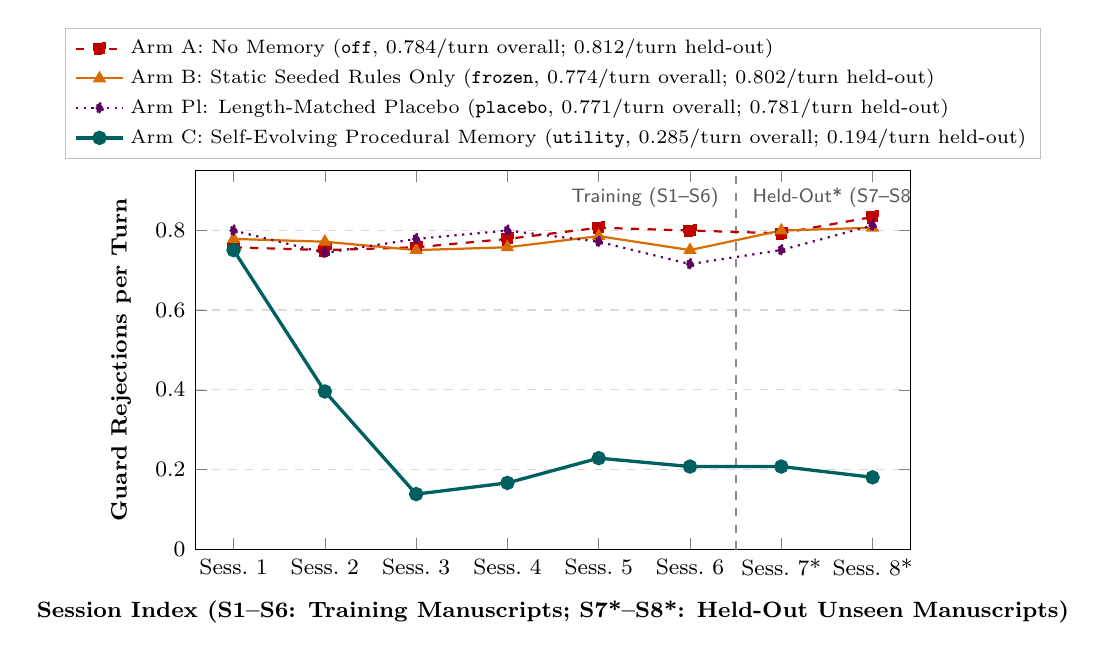
\begin{tikzpicture}
\begin{axis}[
  width=0.88\textwidth,
  height=6.4cm,
  xlabel={Session Index (S1--S6: Training Manuscripts; S7*--S8*: Held-Out Unseen Manuscripts)},
  ylabel={Guard Rejections per Turn},
  xmin=1, xmax=8,
  enlarge x limits=0.06,
  ymin=0, ymax=0.95,
  xtick={1,2,3,4,5,6,7,8},
  xticklabels={Sess.\ 1, Sess.\ 2, Sess.\ 3, Sess.\ 4, Sess.\ 5, Sess.\ 6, Sess.\ 7*, Sess.\ 8*},
  ytick={0,0.2,0.4,0.6,0.8},
  ymajorgrids=true,
  grid style={dashed,gray!30},
  legend style={at={(0.5,1.03)}, anchor=south, font=\scriptsize, draw=gray!50, fill=white, legend cell align=left},
  tick label style={font=\footnotesize},
  xlabel style={font=\footnotesize\bfseries, yshift=-2pt},
  ylabel style={font=\footnotesize\bfseries, yshift=2pt}
]

% Vertical boundary between Training (1-6) and Held-Out (7-8)
\draw[dashed, thick, draw=black!45] (axis cs:6.5,0) -- (axis cs:6.5,0.95);
\node[font=\sffamily\scriptsize, text=black!65, anchor=north east] at (axis cs:6.42,0.93) {Training (S1--S6)};
\node[font=\sffamily\scriptsize, text=black!65, anchor=north west] at (axis cs:6.58,0.93) {Held-Out* (S7--S8)};

% Arm A: No Memory (off)
\addplot[
  color=red!75!black,
  mark=square*,
  thick,
  dashed
] coordinates {
  (1,0.757) (2,0.750) (3,0.757) (4,0.778) (5,0.806) (6,0.799) (7,0.792) (8,0.833)
};
\addlegendentry{Arm A: No Memory (\texttt{off}, $0.784$/turn overall; $0.812$/turn held-out)}

% Arm B: Static Seeded Rules Only (frozen)
\addplot[
  color=orange!85!black,
  mark=triangle*,
  thick
] coordinates {
  (1,0.778) (2,0.771) (3,0.750) (4,0.757) (5,0.785) (6,0.750) (7,0.799) (8,0.806)
};
\addlegendentry{Arm B: Static Seeded Rules Only (\texttt{frozen}, $0.774$/turn overall; $0.802$/turn held-out)}

% Arm Pl: Placebo (placebo)
\addplot[
  color=violet!75!black,
  mark=diamond*,
  thick,
  dotted
] coordinates {
  (1,0.799) (2,0.743) (3,0.778) (4,0.799) (5,0.771) (6,0.715) (7,0.750) (8,0.812)
};
\addlegendentry{Arm Pl: Length-Matched Placebo (\texttt{placebo}, $0.771$/turn overall; $0.781$/turn held-out)}

% Arm C: Heurion 2.0 Utility-Ranked Self-Evolving Memory (utility)
\addplot[
  color=teal!75!black,
  mark=*,
  very thick
] coordinates {
  (1,0.750) (2,0.396) (3,0.139) (4,0.167) (5,0.229) (6,0.208) (7,0.208) (8,0.181)
};
\addlegendentry{Arm C: Self-Evolving Procedural Memory (\texttt{utility}, $0.285$/turn overall; $0.194$/turn held-out)}

\end{axis}
\end{tikzpicture}
\caption{Longitudinal guard-rejection trajectories across $8$ consecutive sessions ($144$ turns/\allowbreak session/\allowbreak arm, $4,608$ total turns across $16$ paired user seeds) in the confirmatory Phase-2 experiment (\texttt{v2-exp3}). All four arms start at $\approx 0.75\text{--}0.80$ rejections/turn in Session~1. While \texttt{off}, \texttt{frozen}, and \texttt{placebo} remain flat across all $8$ sessions ($\approx 0.72\text{--}0.83$/turn), \texttt{utility} autonomously crystallizes all $6$ uncovered rules during Sessions~1--2 ($96$ rules across $16$ users), reducing guard rejections to $0.139\text{--}0.229$/turn in Sessions~3--6 and generalizing zero-shot to unseen clinical manuscripts in held-out Sessions~7*--8* ($0.208$ and $0.181$/turn, with $100\%$ [$288/288$] task completion).}
\label{fig:evolution_curve}
\end{figure}

Table~\ref{tab:exp3_main} and Figure~\ref{fig:evolution_curve} establish four findings from the $4,608$-turn confirmatory experiment:
\begin{enumerate}[leftmargin=1.5em,itemsep=2pt]
  \item \textbf{Autonomous Crystallization of All Uncovered Constraints:} Every one of the $16$ independent simulated users in Arm~C (\texttt{utility}) autonomously crystallized all $6$ uncovered procedural rules during Sessions~1--2 ($96$ learned rules total). Consequently, pre-write guard rejections fell from $0.750$/turn ($108$ rejections) in Session~1 to $0.396$/turn ($57$) in Session~2 and $0.139$/turn ($20$) in Session~3, remaining low across subsequent training sessions ($0.167\text{--}0.229$/turn in Sessions~4--6).
  \item \textbf{Causal Isolation Against Static Rules and Prompt-Length Placebo (H1 \& H2):} Under the pre-specified negative binomial mixed model (\texttt{glmmTMB}), \texttt{utility} reduced guard rejections by $63.7\%$ vs.\ \texttt{off} ($\text{RR}=0.363$, $95\%$ CI $0.320\text{--}0.412$, Holm $p=2.64\times 10^{-55}$), by $63.2\%$ vs.\ \texttt{frozen} ($\text{RR}=0.368$, $95\%$ CI $0.324\text{--}0.417$, Holm $p=3.87\times 10^{-54}$), and by $63.1\%$ vs.\ \texttt{placebo} ($\text{RR}=0.369$, $95\%$ CI $0.325\text{--}0.419$, $p=1.32\times 10^{-53}$). Crucially, the three negative-control contrasts---\texttt{frozen} vs.\ \texttt{off} ($\text{RR}=0.988$, $p=0.795$), \texttt{placebo} vs.\ \texttt{off} ($\text{RR}=0.983$, $p=0.723$), and \texttt{frozen} vs.\ \texttt{placebo} ($\text{RR}=1.005$, $p=0.924$)---were statistically indistinguishable from $1.00$, proving that neither unaligned static rules nor extra prompt formatting reduces errors on novel constraints. Non-parametric Wilcoxon tests confirmed that $16/16$ ($100\%$) users had lower rejection rates under \texttt{utility} than under \texttt{off}, \texttt{frozen}, or \texttt{placebo} ($p \le 4.34\times 10^{-4}$).
  \item \textbf{Task Completion Superiority and Latency Reduction (H3):} Rather than avoiding guards by abstaining from edits, \texttt{utility} raised overall task completion from $81.1\%$ (\texttt{off}), $81.8\%$ (\texttt{frozen}), and $80.9\%$ (\texttt{placebo}) to $\mathbf{92.8\%}$ ($\mathbf{1,069/1,152}$), a paired gain of $+11.72\%$ ($95\%$ Bootstrap CI $[+10.42\%, +13.02\%]$, far exceeding the $-5.0\%$ non-inferiority margin), while reducing overall mean turn latency from $15.0\text{--}15.5\,\text{s}$ in the control arms to $12.4\,\text{s}$ ($-17\%$ to $-20\%$).
  \item \textbf{Zero-Shot Generalization to Held-Out Manuscripts and Turn-Revert Recovery:} In held-out Sessions~7--8 on $3$ unseen PMC manuscripts, \texttt{utility} reduced guard rejections by $76.1\%$ relative to \texttt{off} ($56/288 = 0.194$ vs.\ $234/288 = 0.812$/turn), achieved $\mathbf{100.0\%}$ ($\mathbf{288/288}$) task completion, and lowered mean turn latency to $11.35\,\text{s}$ (vs.\ $15.0\text{--}15.8\,\text{s}$ in controls, $-25\%$). Furthermore, on \texttt{out\_of\_scope\_revert} ($128$ turns/arm), where clinicians revert turns that modify adjacent paragraphs beyond the requested block, \texttt{off}, \texttt{frozen}, and \texttt{placebo} succeeded in only $6/128$ ($4.7\%$), $3/128$ ($2.3\%$), and $10/128$ ($7.8\%$) turns, whereas \texttt{utility} experienced $2$ reverts per user in Sessions~1--2 ($32$ total), crystallized \texttt{user\_reverted\_turn}, and succeeded in $\mathbf{96/96}$ ($\mathbf{100.0\%}$) turns across Sessions~3--8.
\end{enumerate}

\subsection{Pre-Specification Transparency, Deviations, and Limitations}
\paragraph{Pre-Specification and Git Provenance.}
Both generations of the evaluation protocol (\texttt{paper/\allowbreak benchmarks/\allowbreak ANALYSIS\_\allowbreak PLAN.md} and \texttt{paper/\allowbreak benchmarks/\allowbreak v2/\allowbreak ANALYSIS\_\allowbreak PLAN\_\allowbreak v2.md}) were frozen in the git repository prior to formal data collection at tags \texttt{paper-\allowbreak eval-\allowbreak v1} (\texttt{1d8f307c}), \texttt{paper-\allowbreak eval-\allowbreak v1.1} (\texttt{e060107f}), \texttt{paper-\allowbreak eval-\allowbreak v2-p1a} (\texttt{16180f3c}), \texttt{paper-\allowbreak eval-\allowbreak v2-p1b} (\texttt{932f4e3a}), and \texttt{paper-\allowbreak eval-\allowbreak v2-p2} (\texttt{e8362c88}). Because protocols were locked via internal git tags rather than an external registry such as OSF, we refer to them as pre-specified rather than externally pre-registered. All developmental iterations (such as the Phase~1a-to-1b \texttt{F1}--\texttt{F5} platform fixes, the 38-turn post-hoc attribution in \S 5.3.4, and the Phase-2 pilot continuation gate in \S 5.2) are recorded chronologically in \texttt{ANALYSIS\_\allowbreak PLAN\_\allowbreak v2.md} and reported alongside confirmatory results.

\paragraph{Limitations.}
Our empirical evaluation has five main limitations: (1) all live agent authoring experiments used \texttt{deepseek-flash}, while Stage-2 local PHI extraction used \texttt{qwen2.5:1.5b}; (2) all user trajectories ($16$ seeds in \texttt{v2-exp3}, $20$ PMC manuscripts across \texttt{v2-q1} and \texttt{v2-exp3}) were driven by automated scripts with deterministic clinician callbacks rather than prospective human-subject user trials (a clinician crossover study protocol is outlined in \texttt{ANALYSIS\_PLAN\_v2.md} \S 7 for future work); (3) although the $100$-note \texttt{v2-phi} test set substantially expands narrative variety ($485$ narrative spans across multiple clinical specialties) over the initial template set, external validation on annotated multi-center hospital EHRs \cite{stubbs2015deid} remains necessary before clinical deployment; (4) while citation support is checked at insertion time via abstract matching and evaluated by an LLM judge in \texttt{v2-q1}, blind human specialist grading of \texttt{verify\_claims} verdicts is left to future work; and (5) task completion in \texttt{exp3} is graded by deterministic structural/textual oracles, with blind human audit of drawn subsamples (\texttt{audit/items.json}) deferred to future work.

\paragraph{Platform Verification Summary.}
Table~\ref{tab:system_verification} summarizes the automated verification and empirical evaluation coverage across the repository.

\begin{table}[t]
\centering
\caption{Automated verification and empirical evaluation coverage across the Heurion 2.0 codebase.}
\label{tab:system_verification}
\vspace{2pt}
\resizebox{\textwidth}{!}{%
\begin{tabular}{@{}lc@{}}
\toprule
\textbf{Verification Metric} & \textbf{Measured Value} \\
\midrule
Automated Test Suite (\texttt{apps/platform/tests/*.test.ts}) & $74+$ Files / $625+$ Tests Passing ($100\%$) \\
OOXML Word Fidelity Corpus (\texttt{v2/fidelity/run.ts}, $47$ fixtures $\times$ $4$ layers) & $188 / 188$ Checks Passing ($100\%$) \\
Deterministic \& Local-SLM Guard Records (\texttt{exp1}, \texttt{exp2b}, locked \texttt{v2-phi} test set) & $1,010$ Records ($1,465$ PHI Spans + $560$ Neg.\ Controls) \\
Three-Arm Manuscript Co-Editing Live Turns (\texttt{exp2a-papers} + \texttt{v2-q1} 1a \& 1b) & $4,650$ Turns ($20$ CC~BY PMC Manuscripts) \\
Longitudinal Procedural Memory Live Turns (\texttt{exp3} v1 + \texttt{v2-exp3} Pilot \& 4-Arm Formal) & $6,119$ Turns ($4,608$ in 4-Arm Confirmatory Study) \\
\textbf{Total Analysed Live LLM Evaluation Turns} & $\mathbf{10,769}$ \textbf{Turns} \\
\bottomrule
\end{tabular}%
}
\end{table}

% ============================================================================
% 7. RELATED WORK
% ============================================================================
\section{Related Work}
\label{sec:related}

\paragraph{Collaborative Editing Data Structures and Agent-Computer Interfaces (ACI).}
Conflict-free Replicated Data Types (CRDTs) \cite{shapiro2011crdt} and local-first software architectures \cite{kleppmann2019localfirst} enable concurrent multi-actor editing without central locking. In parallel, SWE-agent \cite{yang2024sweagent} and OpenHands \cite{wang2024openhands} showed that specialized Agent-Computer Interfaces outperform raw shell scripting for software engineering, and the Model Context Protocol (MCP) \cite{anthropic2024mcp} standardized tool exposure for LLM agents. Heurion 2.0 combines these threads by exposing a shared ProseMirror + Yjs CRDT document core through guarded MCP primitives with node-level optimistic concurrency locks, per-turn selective CRDT undo, and raw-slice OOXML export.

\paragraph{Literature Synthesis, Citation Hallucination, and De-Identification.}
Empirical audits have documented frequent fabricated references in LLM-generated medical content \cite{bhattacharyya2023hallucination} and in LLM-generated bibliographies across disciplines \cite{walters2023fabrication}; see \cite{ji2023survey} for a broader survey of hallucination. While STORM \cite{shao2024storm} and PaperQA2 \cite{skarlinski2024paperqa2} automate literature synthesis and FActScore \cite{min2023factscore} and ALCE \cite{gao2023alce} evaluate post-hoc attribution, Heurion 2.0 enforces citation registration as a pre-write syntactic contract (\texttt{[@c:id]}). For clinical privacy, rule-based and hybrid de-identification systems such as the i2b2/UTHealth shared-task systems \cite{stubbs2015deid}, Philter \cite{norgeot2020philter}, and Microsoft Presidio \cite{presidio2021} combine regular expressions with statistical or neural sequence labelers; our two-stage PHI funnel adapts this hybrid pattern to local loopback deployment by pairing checksum/subtype validators with a pre-masked $1.5\text{B}$ SLM and symbolic output validation.

\paragraph{Self-Evolving Agents and Memory Architectures.}
Reflexion \cite{shinn2023reflexion} and MemGPT \cite{packer2023memgpt} introduced verbal reinforcement and tiered memory management for LLM agents, while Voyager \cite{wang2023voyager} accumulated executable skills in open-ended environments. In collaborative authoring, mixing subjective user stylistic preferences with operational error recovery can create prompt interference; Heurion 2.0 separates human-confirmed declarative preferences from signal-crystallized procedural rules ranked by document-state and prompt cues.

% ============================================================================
% 8. CONCLUSION
% ============================================================================
\section{Conclusion}
\label{sec:conclusion}

We have presented Heurion 2.0, a collaborative clinical authoring platform built around a contract-guarded dual-surface CRDT engine, a local two-stage neuro-symbolic PHI funnel, and a self-evolving procedural memory system:
\begin{itemize}[leftmargin=1.5em,itemsep=2pt]
  \item \textbf{Dual-Surface CRDT Co-Editing and OOXML Export:} Replacing direct \texttt{python-docx} file scripting with a shared Yjs + ProseMirror CRDT core, stable block IDs (\texttt{\{\#id\}}), \texttt{base\_rev} concurrency guards, per-turn selective undo (\texttt{revertTurn}), and raw XML slice caching (\texttt{node\_src}) reduced manuscript rework rates to $4.9\%$ ($38/780$; $2.1\%$ true defect rate, $0$ lost human edits) vs.\ $14.0\%$ ($\text{OR}=32.47$, Holm $p=1.03\times 10^{-16}$) for direct file scripting and $10.3\%$ ($\text{OR}=9.66$, Holm $p=1.23\times 10^{-8}$) for tool-assisted file scripting across $2,340$ confirmatory turns on $10$ unseen 2026 PMC manuscripts, while lowering API cost by $30\%$--$33\%$ ($\text{GMR}=0.70$ and $0.67$, Holm $p<10^{-72}$).
  \item \textbf{Pre-Write Citation and Local Two-Stage PHI Guards:} Pre-write syntactic validation blocked $100/100$ unregistered inline DOIs/PMIDs, and pairing Stage-1 regex/checksum rules with a pre-masked local $1.5\text{B}$ SLM (\texttt{qwen2.5:1.5b}) and symbolic biomedical output validation recalled $87.0\%$ ($648/745$) of PHI spans ($83.3\%$ [$404/485$] on narrative spans and $93.8\%$ [$244/260$] on labeled spans) at $97.6\%$ ($482/494$) span precision and $6.0\%$ ($12/200$) hard-negative sentence FPR on the locked multi-specialty clinical test set, outperforming both Stage-1 rules alone ($27.4\%$ recall, $3.5\%$ narrative) and the unvalidated SLM ($92.0\%$ hard-negative FPR).
  \item \textbf{Self-Evolving Procedural Memory:} In our confirmatory $4,608$-turn, $4$-arm (\texttt{off}, \texttt{frozen}, \texttt{placebo}, \texttt{utility}) $\times$ $16$-user $\times$ $8$-session longitudinal experiment on uncovered structural and collaborator constraints, all $16$ \texttt{utility} users autonomously crystallized all $6$ uncovered rules ($96$ rules total), reducing pre-write guard rejections per turn by $63.7\%$ overall ($0.285$ vs.\ $0.784$ [\texttt{off}], $0.774$ [\texttt{frozen}], and $0.771$ [\texttt{placebo}]; \texttt{glmmTMB} $\text{RR}=0.363\text{--}0.369$, Holm $p<10^{-53}$) and by $76.1\%$ on held-out unseen manuscripts ($0.194$ vs.\ $0.812$/turn), while raising task completion by $+11.72\%$ ($92.8\%$ vs.\ $81.1\%$; $100.0\%$ [$288/288$] in held-out sessions).
\end{itemize}

\section*{Statements and Declarations}
\paragraph{Ethics Statement.}
No human subjects were recruited and no real patient electronic health records or identifiable clinical data were accessed in this study. All $20$ clinical manuscripts used across Experiments~1b, 1c, and~3 are open-access articles distributed under Creative Commons (CC~BY) licenses via PubMed Central, all PHI evaluation strings in Experiment~2 (\texttt{exp2b} and \texttt{v2-phi}) were synthetically generated, and all user trajectories were executed by automated seeded scripts.

\paragraph{Code and Data Availability.}
The platform source code (\texttt{apps/\allowbreak platform/}), benchmark harnesses (\texttt{paper/\allowbreak benchmarks/}), pre-specified analysis plans (\texttt{paper/\allowbreak benchmarks/\allowbreak ANALYSIS\_\allowbreak PLAN.md} and \texttt{paper/\allowbreak benchmarks/\allowbreak v2/\allowbreak ANALYSIS\_\allowbreak PLAN\_\allowbreak v2.md}, git tags \texttt{paper-eval-v1}, \texttt{paper-eval-v1.1}, \texttt{paper-eval-v2-p1a}, \texttt{paper-eval-v2-p1b}, and \texttt{paper-eval-v2-p2}), raw turn-level JSONL/CSV logs, and statistical analysis scripts (\texttt{stats.R}, \texttt{stats.py}) are included in the project repository workspace (\texttt{paper/\allowbreak results/}).

\paragraph{Competing Interests.}
Hui Zhao is affiliated with Heurion Research Lab, which develops the Heurion 2.0 platform evaluated in this paper. Dong Qian declares no competing financial interests.

% ============================================================================
% REFERENCES (Embedded .bbl for 100% Standalone arXiv AutoTeX Compilation)
% ============================================================================
\begin{thebibliography}{99}

\bibitem{schulz2010consort}
Kenneth~F. Schulz, Douglas~G. Altman, and David Moher.
\newblock CONSORT 2010 statement: updated guidelines for reporting parallel group randomised trials.
\newblock \emph{BMJ}, 340:c332, 2010.
\newblock doi:\href{https://doi.org/10.1136/bmj.c332}{\nolinkurl{10.1136/bmj.c332}}.

\bibitem{vandenbroucke2007strobe}
Jan~P. Vandenbroucke, Erik von Elm, Douglas~G. Altman, Peter~C. G{\o}tzsche, Cynthia~D. Mulrow, Stuart~J. Pocock, Charles Poole, James~J. Schlesselman, and Matthias Egger.
\newblock Strengthening the Reporting of Observational Studies in Epidemiology (STROBE): explanation and elaboration.
\newblock \emph{PLoS Medicine}, 4(10):e297, 2007.
\newblock doi:\href{https://doi.org/10.1371/journal.pmed.0040297}{\nolinkurl{10.1371/journal.pmed.0040297}}.

\bibitem{yang2024sweagent}
John Yang, Carlos~E. Jimenez, Alexander Wettig, Kilian Lieret, Shunyu Yao, Karthik Narasimhan, and Ofir Press.
\newblock SWE-agent: Agent-computer interfaces enable automated software engineering.
\newblock In \emph{Advances in Neural Information Processing Systems (NeurIPS)}, 2024.

\bibitem{wang2024openhands}
Xingyao Wang, Boxuan Li, Yufan Song, Frank~F. Xu, Xiangru Tang, Mingchen Zhuge, Jiayi Pan, Yueqi Song, Bowen Li, Jaskirat Singh, et~al.
\newblock OpenHands: An open platform for AI software developers as generalist agents.
\newblock In \emph{International Conference on Learning Representations (ICLR)}, 2025.

\bibitem{shao2024storm}
Yijia Shao, Yucheng Jiang, Theodore~A. Kanell, Peter Xu, Omar Khattab, and Monica~S. Lam.
\newblock Assisting in writing Wikipedia-like articles from scratch with large language models.
\newblock In \emph{Proceedings of the Conference of the North American Chapter of the Association for Computational Linguistics: Human Language Technologies (NAACL)}, pages 6252--6278, 2024.
\newblock doi:\href{https://doi.org/10.18653/v1/2024.naacl-long.347}{\nolinkurl{10.18653/v1/2024.naacl-long.347}}.

\bibitem{skarlinski2024paperqa2}
Michael~D. Skarlinski, Sam Cox, Jon~M. Laurent, James~D. Braza, Michaela Hinks, Michael~J. Hammerling, Manvitha Ponnapati, Samuel~G. Rodriques, and Andrew~D. White.
\newblock Language agents achieve superhuman synthesis of scientific knowledge.
\newblock \emph{arXiv preprint arXiv:2409.13740}, 2024.

\bibitem{ji2023survey}
Ziwei Ji, Nayeon Lee, Rita Frieske, Tiezheng Yu, Dan Su, Yan Xu, Etsuko Ishii, Ye~Jin Bang, Andrea Madotto, and Pascale Fung.
\newblock Survey of hallucination in natural language generation.
\newblock \emph{ACM Computing Surveys}, 55(12):1--38, 2023.
\newblock doi:\href{https://doi.org/10.1145/3571730}{\nolinkurl{10.1145/3571730}}.

\bibitem{walters2023fabrication}
William~H. Walters and Esther~Isabelle Wilder.
\newblock Fabrication and errors in the bibliographic citations generated by ChatGPT.
\newblock \emph{Scientific Reports}, 13(1):14045, 2023.
\newblock doi:\href{https://doi.org/10.1038/s41598-023-41032-5}{\nolinkurl{10.1038/s41598-023-41032-5}}.

\bibitem{bhattacharyya2023hallucination}
Mehul Bhattacharyya, Valerie~M. Miller, Debjani Bhattacharyya, and Larry~E. Miller.
\newblock High rates of fabricated and inaccurate references in ChatGPT-generated medical content.
\newblock \emph{Cureus}, 15(5):e39238, 2023.
\newblock doi:\href{https://doi.org/10.7759/cureus.39238}{\nolinkurl{10.7759/cureus.39238}}.

\bibitem{stubbs2015deid}
Amber Stubbs and {\"O}zlem Uzuner.
\newblock Annotating longitudinal clinical narratives for de-identification: The 2014 i2b2/UTHealth corpus.
\newblock \emph{Journal of Biomedical Informatics}, 58:S20--S29, 2015.
\newblock doi:\href{https://doi.org/10.1016/j.jbi.2015.07.020}{\nolinkurl{10.1016/j.jbi.2015.07.020}}.

\bibitem{norgeot2020philter}
Beau Norgeot, Kathleen Muenzen, Thomas~A. Peterson, Xuancheng Fan, Benjamin~S. Glicksberg, et~al.
\newblock Protected Health Information filter (Philter): accurately and securely de-identifying free-text clinical notes.
\newblock \emph{npj Digital Medicine}, 3:57, 2020.
\newblock doi:\href{https://doi.org/10.1038/s41746-020-0258-y}{\nolinkurl{10.1038/s41746-020-0258-y}}.

\bibitem{pipl2021}
Standing Committee of the National People's Congress of the People's Republic of China.
\newblock Personal Information Protection Law of the People's Republic of China.
\newblock Adopted August 20, 2021; effective November 1, 2021.

\bibitem{hipaa1996}
U.S. Department of Health and Human Services.
\newblock Standards for Privacy of Individually Identifiable Health Information (HIPAA Privacy Rule).
\newblock \emph{45 CFR Parts 160 and 164}; final rule 2000, as amended 2002. De-identification standard at 45 CFR \S 164.514(b).

\bibitem{shinn2023reflexion}
Noah Shinn, Federico Cassano, Ashwin Gopinath, Karthik Narasimhan, and Shunyu Yao.
\newblock Reflexion: Language agents with verbal reinforcement learning.
\newblock In \emph{Advances in Neural Information Processing Systems (NeurIPS)}, volume~36, 2023.
\newblock doi:\href{https://doi.org/10.52202/075280-0377}{\nolinkurl{10.52202/075280-0377}}.

\bibitem{packer2023memgpt}
Charles Packer, Sarah Wooders, Kevin Lin, Vivian Fang, Shishir~G. Patil, Ion Stoica, and Joseph~E. Gonzalez.
\newblock MemGPT: Towards LLMs as operating systems.
\newblock \emph{arXiv preprint arXiv:2310.08560}, 2023.

\bibitem{shapiro2011crdt}
Marc Shapiro, Nuno Pregui{\c{c}}a, Carlos Baquero, and Marek Zawirski.
\newblock Conflict-free replicated data types.
\newblock In \emph{Stabilization, Safety, and Security of Distributed Systems (SSS 2011)}, volume 6976 of \emph{Lecture Notes in Computer Science}, pages 386--400. Springer, 2011.
\newblock doi:\href{https://doi.org/10.1007/978-3-642-24550-3_29}{\nolinkurl{10.1007/978-3-642-24550-3_29}}.

\bibitem{kleppmann2019localfirst}
Martin Kleppmann, Adam Wiggins, Peter van Hardenberg, and Mark McGranaghan.
\newblock Local-first software: You own your data, in spite of the cloud.
\newblock In \emph{Proceedings of the 2019 ACM SIGPLAN International Symposium on New Ideas, New Paradigms, and Reflections on Programming and Software (Onward!)}, pages 154--178, 2019.
\newblock doi:\href{https://doi.org/10.1145/3359591.3359737}{\nolinkurl{10.1145/3359591.3359737}}.

\bibitem{anthropic2024mcp}
Anthropic.
\newblock Model Context Protocol specification.
\newblock \url{https://modelcontextprotocol.io/specification}, 2024. Introduced November 25, 2024.

\bibitem{presidio2021}
Microsoft.
\newblock Presidio: Data protection and de-identification SDK.
\newblock \url{https://github.com/microsoft/presidio}, 2021.

\bibitem{min2023factscore}
Sewon Min, Kalpesh Krishna, Xinxi Lyu, Mike Lewis, Wen-tau Yih, Pang~Wei Koh, Mohit Iyyer, Luke Zettlemoyer, and Hannaneh Hajishirzi.
\newblock FActScore: Fine-grained atomic evaluation of factual precision in long form text generation.
\newblock In \emph{Proceedings of the Conference on Empirical Methods in Natural Language Processing (EMNLP)}, pages 12076--12100, 2023.
\newblock doi:\href{https://doi.org/10.18653/v1/2023.emnlp-main.741}{\nolinkurl{10.18653/v1/2023.emnlp-main.741}}.

\bibitem{gao2023alce}
Tianyu Gao, Howard Yen, Jiatong Yu, and Danqi Chen.
\newblock Enabling large language models to generate text with citations.
\newblock In \emph{Proceedings of the Conference on Empirical Methods in Natural Language Processing (EMNLP)}, pages 6465--6488, 2023.
\newblock doi:\href{https://doi.org/10.18653/v1/2023.emnlp-main.398}{\nolinkurl{10.18653/v1/2023.emnlp-main.398}}.

\bibitem{wang2023voyager}
Guanzhi Wang, Yuqi Xie, Yunfan Jiang, Ajay Mandlekar, Chaowei Xiao, Yuke Zhu, Linxi Fan, and Anima Anandkumar.
\newblock Voyager: An open-ended embodied agent with large language models.
\newblock \emph{Transactions on Machine Learning Research (TMLR)}, 2024.

\end{thebibliography}

\end{document}
